%%%%%%%%%%%%%%%%%%%%%%%%%%%%%%%%%%%%%%%%%%%%%%%%%%%%%%%%%%%%%%%%%%%%%%%%%%%%%
%%%
%%% File: thesis.tex, version 1.9, May 2016
%%%
%%% =============================================
%%% This file contains a template that can be used with the package
%%% cs.sty and LaTeX2e to produce a thesis that meets the requirements
%%% of the Computer Science Department from the Technical University of Cluj-Napoca
%%%%%%%%%%%%%%%%%%%%%%%%%%%%%%%%%%%%%%%%%%%%%%%%%%%%%%%%%%%%%%%%%%%%%%%%%%%%%

\documentclass[12pt,a4paper,twoside]{report}         
\usepackage{cs}              
\usepackage{times}
\usepackage{graphicx}
\usepackage{latexsym}
\usepackage{amsmath,amsbsy}
\usepackage{amssymb}
\usepackage[matrix,arrow]{xy}
\usepackage[T1]{fontenc}
\usepackage{ae,aecompl}
\usepackage{romanian} %definitii pentru diacritice; 
\usepackage{amstext}
\usepackage{graphics}
\usepackage[T1]{fontenc}
\usepackage{ae,aecompl}
\usepackage{algorithm}
%\usepackage{algorithmic}
\usepackage{color}
\usepackage{color}
\usepackage{listings}
\usepackage{array,longtable}

\usepackage{color}
\definecolor{lightgray}{rgb}{0.95, 0.95, 0.95}
\definecolor{darkgray}{rgb}{0.4, 0.4, 0.4}
%\definecolor{purple}{rgb}{0.65, 0.12, 0.82}
\definecolor{editorGray}{rgb}{0.95, 0.95, 0.95}
\definecolor{editorOcher}{rgb}{1, 0.5, 0} % #FF7F00 -> rgb(239, 169, 0)
\definecolor{editorGreen}{rgb}{0, 0.5, 0} % #007C00 -> rgb(0, 124, 0)
\definecolor{orange}{rgb}{1,0.45,0.13}		
\definecolor{olive}{rgb}{0.17,0.59,0.20}
\definecolor{brown}{rgb}{0.69,0.31,0.31}
\definecolor{purple}{rgb}{0.38,0.18,0.81}
\definecolor{lightblue}{rgb}{0.1,0.57,0.7}
\definecolor{lightred}{rgb}{1,0.4,0.5}
\usepackage{upquote}
\usepackage{listings}
\usepackage[acronym,nonumberlist, toc]{glossaries}
\usepackage[utf8]{inputenc}
\newglossaryentry{blockchain}
{
    name=blockchain,
    description={baz'a de date distribuit'a, 'intre'tinut'a de o serie de participan'ti care valideaz'a 'inregistr'arile din cadrul re'telei folosind comunicare peer-to-peer}
}

\newglossaryentry{hyperledger fabric}
{
    name=Hyperledger Fabric,
    description={framework pentru implementarea unei re'tele blockchain}
}

\newglossaryentry{CRUD}
{
    name=CRUD,
    description={Create, Read, Update, Delete. }
}

\newglossaryentry{REST}
{
    name=REST,
    description={REpresentational State Transfer Endpoint. Stil arhitectural pentru servicii bazate pe protocolul HTTP}
}

\newglossaryentry{HTTP}
{
    name=HTTP,
    description={HyperText Transfer Protocol. Protocol pentru transmiterea de mesaje}
}

\newglossaryentry{peer-to-peer}
{
    name=peer-to-peer,
    description={Arhitectura de re'tea pentru aplica'tii distribuite}
}

\newglossaryentry{JSON}
{
    name=JSON,
    description={JavaScript Object Notation. Format folosit pentru schimbul de informa'tii 'intre diferite sisteme}
}

\newglossaryentry{BNA}
{
    name=BNA,
    description={Business Network Archive. Implementarea cazurilor de utilizare 'intr-o re'tea blockchain Hyperledger Fabric}
}

\newglossaryentry{API}
{
    name=API,
    description={Application Programming Interface. Set de func'tii 'si metode cu rol 'in stabilirea unui contract 'intre diferite programe pentru realizarea comunic'arii}
}

\makenoidxglossaries


% CSS
\lstdefinelanguage{CSS}{
  keywords={color,background-image:,margin,padding,font,weight,display,position,top,left,right,bottom,list,style,border,size,white,space,min,width, transition:, transform:, transition-property, transition-duration, transition-timing-function},	
  sensitive=true,
  morecomment=[l]{//},
  morecomment=[s]{/*}{*/},
  morestring=[b]',
  morestring=[b]",
  alsoletter={:},
  alsodigit={-}
}

% JavaScript
\lstdefinelanguage{JavaScript}{
  morekeywords={typeof, new, true, false, catch, function, return, null, catch, switch, var, if, in, while, do, else, case, break},
  morecomment=[s]{/*}{*/},
  morecomment=[l]//,
  morestring=[b]",
  morestring=[b]'
}

\lstdefinelanguage{HTML5}{
  language=html,
  sensitive=true,	
  alsoletter={<>=-},	
  morecomment=[s]{<!-}{-->},
  tag=[s],
  otherkeywords={
  % General
  >,
  % Standard tags
	<!DOCTYPE,
  </html, <html, <head, <title, </title, <style, </style, <link, </head, <meta, />,
	% body
	</body, <body,
	% Divs
	</div, <div, </div>, 
	% Paragraphs
	</p, <p, </p>,
	% scripts
	</script, <script,
  % More tags...
  <canvas, /canvas>, <svg, <rect, <animateTransform, </rect>, </svg>, <video, <source, <iframe, </iframe>, </video>, <image, </image>, <header, </header, <article, </article
  },
  ndkeywords={
  % General
  =,
  % HTML attributes
  charset=, src=, id=, width=, height=, style=, type=, rel=, href=,
  % SVG attributes
  fill=, attributeName=, begin=, dur=, from=, to=, poster=, controls=, x=, y=, repeatCount=, xlink:href=,
  % properties
  margin:, padding:, background-image:, border:, top:, left:, position:, width:, height:, margin-top:, margin-bottom:, font-size:, line-height:,
	% CSS3 properties
  transform:, -moz-transform:, -webkit-transform:,
  animation:, -webkit-animation:,
  transition:,  transition-duration:, transition-property:, transition-timing-function:,
  }
}

\lstdefinestyle{htmlcssjs} {%
  % General design
%  backgroundcolor=\color{editorGray},
  basicstyle={\footnotesize\ttfamily},   
  frame=b,
  % line-numbers
  xleftmargin={0.75cm},
  numbers=left,
  stepnumber=1,
  firstnumber=1,
  numberfirstline=true,	
  % Code design
  identifierstyle=\color{black},
  keywordstyle=\color{blue}\bfseries,
  ndkeywordstyle=\color{editorGreen}\bfseries,
  stringstyle=\color{editorOcher}\ttfamily,
  commentstyle=\color{brown}\ttfamily,
  % Code
  language=HTML5,
  alsolanguage=JavaScript,
  alsodigit={.:;},	
  tabsize=2,
  showtabs=false,
  showspaces=false,
  showstringspaces=false,
  extendedchars=true,
  breaklines=true,
  % German umlauts
  literate=%
  {Ö}{{\"O}}1
  {Ä}{{\"A}}1
  {Ü}{{\"U}}1
  {ß}{{\ss}}1
  {ü}{{\"u}}1
  {ä}{{\"a}}1
  {ö}{{\"o}}1
}
%
\lstdefinestyle{py} {%
language=python,
literate=%
*{0}{{{\color{lightred}0}}}1
{1}{{{\color{lightred}1}}}1
{2}{{{\color{lightred}2}}}1
{3}{{{\color{lightred}3}}}1
{4}{{{\color{lightred}4}}}1
{5}{{{\color{lightred}5}}}1
{6}{{{\color{lightred}6}}}1
{7}{{{\color{lightred}7}}}1
{8}{{{\color{lightred}8}}}1
{9}{{{\color{lightred}9}}}1,
basicstyle=\footnotesize\ttfamily, % Standardschrift
numbers=left,               % Ort der Zeilennummern
%numberstyle=\tiny,          % Stil der Zeilennummern
%stepnumber=2,               % Abstand zwischen den Zeilennummern
numbersep=5pt,              % Abstand der Nummern zum Text
tabsize=4,                  % Groesse von Tabs
extendedchars=true,         %
breaklines=true,            % Zeilen werden Umgebrochen
keywordstyle=\color{blue}\bfseries,
frame=b,
commentstyle=\color{brown}\itshape,
stringstyle=\color{editorOcher}\ttfamily, % Farbe der String
showspaces=false,           % Leerzeichen anzeigen ?
showtabs=false,             % Tabs anzeigen ?
xleftmargin=17pt,
framexleftmargin=17pt,
framexrightmargin=5pt,
framexbottommargin=4pt,
%backgroundcolor=\color{lightgray},
showstringspaces=false,      % Leerzeichen in Strings anzeigen ?
}%
%
\makeatother

% \mastersthesis
\diplomathesis
% \leftchapter
\centerchapter
% \rightchapter
\singlespace
% \oneandhalfspace
% \doublespace

\renewcommand{\thesisauthor}{Alin Dan 'TANDEA}    %% Your name.
\renewcommand{\thesismonth}{Iunie}     %% Your month of graduation.
\renewcommand{\thesisyear}{2018}      %% Your year of graduation.
\renewcommand{\thesistitle}{Managementul studiilor clinice bazat pe
tehnologia blockchain} % Title
\renewcommand{\thesissupervisor}{asis. Ing. Cosmina Ivan}
\newcommand{\department}{FACULTATEA DE AUTOMATIC'A 'SI CALCULATOARE\\
DEPARTAMENTUL CALCULATOARE}
\newcommand{\thesis}{LUCRARE DE LICEN'T'A}
\newcommand{\uline}[1]{\rule[0pt]{#1}{0.4pt}}
%\renewcommand{\thesisdedication}{P'arin'tilor mei}
\newcommand{\utcnlogo}{
\includegraphics[width=15cm]{img/utcn.jpg}}

\begin{document}
%\frontmatter
%\pagestyle{headings}

\newenvironment{definition}[1][Defini'tie.]{\begin{trivlist}
\item[\hskip \labelsep {\bfseries #1}]}{\end{trivlist}}





%\thesistitle                    %% Generate the title page.
%\authordeclarationpage                %% Generate the declaration page.

\pagenumbering{arabic}
\setcounter{page}{4}



\begin{center}
%\includegraphics[width=15cm]{img/tucn.jpg}  
\utcnlogo

{\bf \department}

\vspace{4cm}

{\bf \thesistitle} %LICENSE THESIS TITLE}

\vspace{1.5cm}

\thesis

\vspace{6cm}

Absolvent: {\bf \thesisauthor} 

Conduc'ator 'stiin'tific: {\bf \thesissupervisor}

\vspace{3cm}
{\bf \thesisyear}
\end{center}

\thispagestyle{empty}
\newpage

\begin{center}
\utcnlogo

{\bf \department}
\end{center}
\vspace{0.5cm}

%\begin{small}
\begin{tabular}{p{7cm}p{8cm}}
 %\hspace{-1cm}& VIZAT,\\
 \hspace{-1cm}DECAN, & DIRECTOR DEPARTAMENT,\\
\hspace{-1cm}{\bf Prof. dr. ing. Liviu MICLEA} & {\bf Prof. dr. ing. Rodica POTOLEA}\\  
\end{tabular}
 
\vspace{2cm}

\begin{center}
Absolvent: {\bf \thesisauthor}

\vspace{1cm}

{\bf \thesistitle}
\end{center}

\vspace{1cm}

\begin{enumerate}
 \item {\bf Enun'tul temei:} {\it Scopul principal al acestui proiect const'a 'in implementarea unui sistem de management al studiilor clinice cu rol 'in simplificarea activit'a'tii cercet'atorilor din domeniul medical 'si a institu'tiilor de reglementare din domeniu.}
\item {\bf Con'tinutul lucr'arii:} {\it : Cuprins, Lista figurilor, Lista tabelelor, Glosar, Introducere, Obiectivele proiectului,
Studiu bibliografic, Analiz'a 'si Fundamentare teoretic'a, Proiectare de detaliu 'si
implementare, Testare 'si Validare, Manual de instalare 'si utilizare, Concluzii,
Bibliografie, Anexa.}
\item {\bf Locul document'arii:} {\it  Universitatea Tehnic'a din Cluj-Napoca, Departamentul Calculatoare.}
\item {\bf Consultan'ti:} \thesissupervisor
\item {\bf Data emiterii temei:} 1 Noiembrie 2017
\item {\bf Data pred'arii:} 9 Iulie 2018 
  \end{enumerate}
\vspace{1.2cm}

\hspace{6cm} Absolvent: \uline{6cm} 

\vspace{0.5cm}
\hspace{6cm} Coordonator 'stiin'tific: \uline{5cm} 
%\end{small}

\thispagestyle{empty}


\newpage
$ $
%\begin{center}
%\utcnlogo

%{\bf \department}
%\end{center}

\thispagestyle{empty}
\newpage

\begin{center}
\utcnlogo

{\bf \department}
\end{center}

\vspace{0.5cm}

\begin{center}
{\bf
Declara'tie pe proprie r'aspundere privind\\ 
autenticitatea lucr'arii de licen't'a}
\end{center}
\vspace{1cm}



Subsemnatul(a)
\underline{\thesisauthor}, 
legitimat('a) cu \underline{CI} seria \underline{MS} nr. 
\underline{872595}
CNP \underline{1951130261719}, autorul lucr'arii \underline{MANAGEMENTUL STUDIILOR CLINICE BAZAT PE }\\\underline{TEHNOLOGIA BLOCKCHAIN}
elaborat'a 'in vederea sus'tinerii examenului de finalizare a studiilor de licen't'a la Facultatea de Automatic'a 'si Calculatoare, Specializarea \underline{Calculatoare} din cadrul Universit'a'tii Tehnice din Cluj-Napoca, sesiunea \underline{Iulie} a anului universitar \underline{2018}, declar pe proprie r'aspundere, c'a aceast'a lucrare este rezultatul propriei activit'a'ti intelectuale, pe baza cercet'arilor mele 'si pe baza informa'tiilor ob'tinute din surse care au fost citate, 'in textul lucr'arii 'si 'in bibliografie.

Declar, c'a aceast'a lucrare nu con'tine por'tiuni plagiate, iar sursele bibliografice au fost folosite cu respectarea legisla'tiei rom\ia ne 'si a conven'tiilor interna'tionale privind drepturile de autor.

Declar, de asemenea, c'a aceast'a lucrare nu a mai fost prezentat'a 'in fa'ta unei alte comisii de examen de licen't'a.

'In cazul constat'arii ulterioare a unor declara'tii false, voi suporta sanc'tiunile administrative, respectiv, \emph{anularea examenului de licen't'a}.

\vspace{1.5cm}

Data \hspace{8cm} Nume, Prenume

\vspace{0.5cm}

\uline{3cm} \hspace{5.9cm} \underline{\thesisauthor}

\vspace{1cm}
\hspace{9.4cm}Semn'atura

\thispagestyle{empty}

\newpage


%\listoftables
%\listoffigures

%\clearpage 
%\newpage

%\begin{comment}
%{\color{red}{\bf De citit 'inainte} (aceast'a pagin'a se va elimina din versiunea final'a)}:
\begin{enumerate}
 \item Cele trei pagini anterioare (foaie de cap'at, foaie sumar, declara'tie) se vor lista pe foi separate (nu fa't'a-verso), fiind incluse 'in lucrarea listat'a. 
 Foaia de sumar (a doua) necesit'a semn'atura absolventului, respectiv a coordonatorului.
 Pe declara'tie se trece data c\ia nd se pred'a lucrarea la secretarii de comisie.
 \item Pe foaia de cap'at, se va trece corect titulatura cadrului didactic 'indrum'ator, 'in englez'a (consulta'ti pagina de unde a'ti desc'arcat acest document pentru lista cadrelor didactice cu titulaturile lor).
 \item Documentul curent {\bf nu} a fost creat 'in MS Office. E posibil sa fie mici diferen'te de formatare. 
\item Cuprinsul 'incepe pe pagina nou'a, impar'a (dac'a se face listare fa't'a-verso), prima pagin'a din capitolul Introducere tot a'sa, fiind numerotat'a cu 1. % Pentru actualizarea cuprinsului, click dreapta pe cuprins (zona cuprinsului va apare cu gri), Update field-$>$Update entire table.
\item Vizualiza'ti (recomandabil 'si 'in timpul edit'arii) acest document % după ce activaţi vizualizarea simbolurilor ascunse de formatare (apăsaţi simbolul  din Home/Paragraph).
\item Fiecare capitol 'incepe pe pagin'a nou'a. % datorită simbolului ascuns Section Break (Next Page) care este deja introdus la capitolul precedent. Dacă ştergeţi din greşeală simbolul, se reintroduce (Page Layout -> Breaks).
\item Folosi'ti stilurile predefinite (Headings, Figure, Table, Normal, etc.)
\item Marginile la pagini nu se modific'a.
\item Respecta'ti restul instruc'tiunilor din fiecare capitol.
\end{enumerate}
 
%\end{comment}

\newpage

\tableofcontents
\newpage
\listoffigures
\listoftables

\renewcommand*{\glossaryname}{Glosar}
\glsaddall
\printnoidxglossaries



\chapter{Introducere - Contextul proiectului}
\pagestyle{headings}
    La momentul actual, domeniul medical beneficiaz'a pe deplin de instumentele digitale puse la dispozi'tie pentru a oferi servicii pacien'tilor. Instrumentele digitale au dus la simplificarea procedurilor 'si metodologiilor din domeniu. 'In ultimii ani institu'tiile medicale au 'inceput s'a renun'te la 'inregistr'arile stocate 'in format fizic 'si au adoptat 'inregistr'ari digitale. Aceasta abordare cre'ste eficien'ta personalului medical, simplific'a activitatea acestora 'si necesita mai putin spa'tiu pentru stocarea informa'tiilor. Totu'si, odat'a cu adoptarea uneltelor digitale, apar 'si 'ingrijor'arile cu privire la siguran'ta datelor cu caracter personal ale pacien'tilor.
    

\section{Contextul proiectului}
    Studiile clinice reprezint'a o parte important'a a cercet'arii 'in domeniul medical. Aceasta parte din cercetarea medical'a presupune implicarea pacien'tilor pentru testarea anumitor tratamente. Aceste tratamente pot fi fie un medicament nou, o procedura medical'a nou'a sau un dispozitiv medical. Scopul studiilor clinice este de a oferi cercet'atorilor posibilitatea de a evalua eficien'ta 'si siguran'ta acestor noi tratamente. De cele mai multe ori studiile clinice sunt folosite pentru a determina dac'a un anumit medicament este mai eficient dec\^at altul deja existent pentru o anumit'a boal'a sau dac'a un medicament are mai pu'tine efecte secundare.
    
    Importan'ta acestui domeniu reiese 'si din investi'tiile atrase 'in acest domeniu. Anual, domeniul studiilor clinice atrage investi'tii majore. 'In anul 2016 industria studiilor clinice era evaluat'a la 40.0 de miliarde de dolari, fiind estimat ca pan'a 'in anul 2025 s'a ajung'a la 65.2 miliarde. Din acest motiv, exist'a riscul apari'tiei fraudelor sau al falsific'arii datelor colectate 'in cadrul unui studiu clinic.
    
    Exist'a numeroase platforme care au ca scop simplificarea metodologiilor din cadrul unui studiu clinic. Acestea simplific'a activit'a'ti precum planificarea studiilor clinice, managementul pacien'tilor 'inrolati sau colectarea de date. Aceste 'inregistr'ari au o importan'ta major'a 'in cadrul cercetarii clinice 'si al reglement'arii acestora. De aceea, sistemele folosite trebuie s'a asigure corectitudinea datelor colectate 'si s'a reduc'a riscul de falsificare al acestora.
    
\section{Con'tinutul lucr'arii}
    
    Aceasta sec'tiune prezint'a structura documentului de licen'ta. Documentul este structurat pe urmatoarele capitole:
    
    \subsubsection{Capitolul 1(Introducere)}
    Primul capitol al lucr'arii are ca scop identificarea contextului temei propuse. Sunt preentate aspecte generale legate de subiect al'aturi de dificult'a'tile 'int\^alnite 'in domeniu. Pe langa aceste aspecte, se prezint'a pe scurt con'tinutul acestui document.
    
    \subsubsection{Capitolul 2(Obiectivele Proiectului)}
    Obiectivele principale 'si secundare ale proiectului al'aturi de motiva'tia pentru alegerea temei lucr'arii sunt prezentate 'in acest capitol.
    
    \subsubsection{Capitolul 3(Studiu Bibliografic)}
    Tehnologia blockchain se afla la baza sistemului implementat. De aceea, acest capitol prezint'a o analiz'a a particularit'a'tilor tehnologiei 'si a relevan'tei acestora pentru domeniul studiilor clinice. Sunt prezentate implement'ari ale tehnologiei al'aturi de o compara'tie a avantajelor 'si dezavantajelor oferite de aceste implement'ari, cu aplicare pe domeniul studiilor clinice.
    
    \subsubsection{Capitolul 4(Analiz'a 'si Fundamentare Teoretic'a)}
    'In acest capitol sunt prezentate cerin'tele func'tionale 'si non-func'tionale specifice unui sistem pentru managementul studiilor clinice. Sunt prezenta'ti principalii actori din sistem al'aturi de cazurile de utilizare asociate fiec'aruia. Capitolul se 'incheie prin prezentarea pe scurt a tehnologiilor 'si uneltelor utilizate pentru implementarea unui sistem care sa 'indeplineasca cerintele func'tionale 'si non-func'tionale impuse.
    
    \subsubsection{Capitolul 5(Proiectare de Detaliu 'si Implementare)}
    Componentele principale ale sistemului 'si interac'tiunea dintre acestea sunt prezentate 'in acest capitol. Capitolul descrie modul de implementare al defini'tiei unei re'tele blockchain, unele fluxuri de executie precum 'si o descriere a componentelor interfe'tei utilizator.
    
    \subsubsection{Capitolul 6(Testare 'si Validare)}
    Definirea unor procese de testare este necesar'a pentru a asigura calitatea sistemului implementat. Acest capitol prezint'a uneltele de testare puse la dispozi'tie pentru testarea unei re'tele blockchain, a punctelor de acces 'in re'tea 'si ale aplica'tiei client.
    
    \subsubsection{Capitolul 7(Manual de Instalare 'si Utilizare)}
    Capitolul descrie dependin'tele hardware 'si software ale sistemului implementat. Sunt descri'si pa'sii necesari pentru punerea 'in func'tiune a componentelor sistemului. Capitolul con'tine, de asemenea un manual de utilizare al aplica'tiei cu scopul de a familiariza utilizatorii cu aplica'tia client a sistemului.
    
    \subsubsection{Capitolul 8(Concluzii)}
    Capitolul con'tine o analiza critic'a asupra avantajelor 'si dezavantajelor aduse de sistemul implementat. Sunt prezentate, de asemenea posibilit'a'tile de 'imbunatatire 'si extindere a sistemului.



\newpage
\thispagestyle{empty}
\mbox{}

\chapter{Obiectivele Proiectului}

\section{Obiective principale}

Obiectivul principal al lucr'arii este implementarea unui sistem distribuit pentru managementul studiilor clinice cu scopul de a simplifica munca entit'a'tilor implicate 'in activit'a'tile din cadrul studiilor clinice 'si al celor responsabile de aplicarea reglement'arilor specifice domeniului. 'In acest sens, obiectivele specifice necesare atingerii obiectivului principal sunt:
    \begin{enumerate}
        \item Dezvoltarea unui sistem care ofer'a posibilitatea desf'a'surarii activitatilor din cadrul unui studiu clinic precum: managementul pacien'tilor, specificarea responsabilit'a'tilor utilizatorilor implica'ti.
        \item Implementarea unui mecanism de colectare a datelor flexibil. Utilizatorilor li se ofer'a flexibilitatea de a defini formulare de colectare a datelor specifice nevoilor 'int'alnite intr-un studiu clinic.
        \item Facilitarea accesului entit'a'tilor responsabile de reglementarea studiilor clinice. Aceasta presupune implementarea unui mecanism care s'a furnizeze utilizatorilor istoricul 'in timp al activit'a'tilor din cadrul studiilor clinice.
    \end{enumerate}
    
\section{Obiective secundare}

    Unul dintre obiectivele secundare ale sistemului este controlul accesului utilizatorilor la serviciile oferite de sistem. Mecanismul de autentificare al utilizatorilor trebuie s'a ofere accesul la resurse doar utilizatorilor care au drepturile necesare definite 'in regulile de acces ale sistemului.
    Sunt definite 4 tipuri de utilizatori ai aplica'tiei:
    \begin{itemize}
        \item Administrator: Responsabil de emiterea 'si revocarea identit'a'tii celorlalti utilizatori din sistem. 
        \item Cercet'ator: Folose'ste func'tionalit'a'tile pentru managementul studiilor clinice oferite de sistem. 
        \item Agent de reglementare: Supervizeaz'a activit'a'tile din cadrul unui studiu clinic. Utilizeaz'a istoricul 'in timp al activit'a'tilor din cadrul unui studiu clinic pentru a-'si 'indeplini obiectivele.
        \item Sponsor: Interesat de rezultatele ob'tinute 'in cadrul unui studiu clinic. Poate vizualiza rapoarte legate de activitatea din studiile clinice.
    \end{itemize}
    
    Managementul identit'a'tii participan'tilor este de asemenea unul din obiectivele sistemului implementat. Fiecare utilizator al sistemului folose'ste cheia asociat'a identit'a'tii lor pentru a autoriza opera'tiile 'in cadrul sistemului. 'In acest fel este posibil'a generarea unui istoric 'in timp al activit'a'tilor din sistem, al'aturi de utilizatorii responsabili de aceste activit'a'ti.
    
    Protec'tia datelor cu caracter personal ale pacien'tilor este un alt obiectiv al sistemului implementat. Utilizatorilor le este permis accesul doar la resursele de care au nevoie pentru a-'si desf'a'sura activitatea. Aplica'tia utilizeaz'a liste de acces care definesc regulile de citire 'si scriere asociate participan'tilor defini'ti anterior asupra resurselor sistemului. 'In acest fel este asigurat'a protec'tia datelor f'ar'a a fi afectat'a activitatea utilizatorilor aplica'tiei.
    
    Un alt obiectiv este folosirea unei arhitecturi distribuite, sub forma unei re'tele de participan'ti 'in care fiecare contribuie la memorarea 'si validarea datelor din sistem. Fiecare nod din re'tea de'tine o copie a informa'tiilor, fiind astfel dificil'a falsificarea datelor f'ar'a ca aceasta s'a fie observat'a de ceilal'ti participan'ti. Redundan'ta asigur'a de asemenea toleran'ta la erori prin eliminarea punctului unic de e'sec.
    
    
    




\chapter{Studiu Bibliografic}
	'In acest capitol sunt prezentate o serie de concepte 'si tehnologii necesare pentru o mai bun'a 'in'telegere a temei alese 'si a modului 'in care au fost utilizate pentru implementarea sistemului. Capitolul continu'a prin descrierea aplic'arii acestor concepte 'in anumite domenii precum 'si 'in domeniul studiilor clinice. Sunt prezentate unele beneficii aduse de aceste tehnologii, al'aturi de o compara'tie a implement'arilor existente ale acesteia.
	\section{Blockchain}	
	Termenul de blockchain a devenit cunoscut odat'a cu cre'sterea 'in popularitate a monedelor virtuale, 'in special a monedei virtuale Bitcoin\footnote{https://bitcoin.org}. O re'tea blockchain poate fi definit'a ca fiind o baza de date distribuit'a, intre'tinut'a de o serie de participan'ti care valideaz'a inregistr'arile din cadrul re'telei folosind o comunicare de tip peer-to-peer. 'Inregistr'arile din cadrul re'telei sunt securizate prin metode criptografice care asigur'a imutabilitatea datelor. Rezolvarea conflictelor care pot ap'area 'intre 'inregistr'arile din re'tea are loc prin utilizarea unor algoritmi de consens. Aceasta sec'tiune analizeaz'a urmatoarele aspecte ale tehnologiei: structura de date, aspecte legate de criptografie, topologia re'telei, algoritmi de consens, smart contracts, permisiuni 'si implement'ari ale tehnologiei.

	\subsection{Structura de date}
	Structura de date folosit'a reprezint'a unul dintre mijloacele care asigur'a integritatea datelor din re'teaua blockchain. Documenta'tia monedei virtuale Bitcoin descrie structura de date folosit'a ca fiind o list'a invers inl'an'tuita 'in care fiecare element, numit bloc, con'tine hash-ul blocului anterior, un timestamp 'si r'ad'acina unui arbore Merkle \cite{merkle}. Frunzele arborelui sunt hash-uri ale tranzac'tiilor iar nodurile din arbore sunt hash-uri ale nodurilor fiu. 'In acest fel este asigurat'a integritatea tranzac'tiilor din structura de date. Figura \ref{fig:btc} prezint'a structura de date folosit'a de Bitcoin\cite{bitcoin}.
	
		\begin{figure}[H]
		\begin{center}
			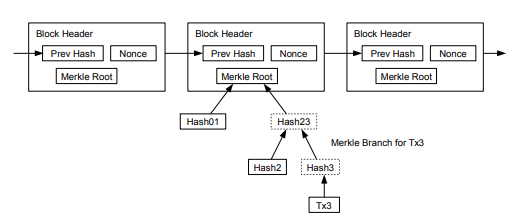
\includegraphics[scale=2.5]{img/btc.png}
			\caption{Lan't proof-of-work folosit de Bitcoin\cite{bitcoin}}
  			\label{fig:btc}
  		\end{center}
  		\end{figure} 
	
	
	
	Fiecare bloc din structura de date este identificat prin func'tia hash a header-ului blocului curent 'si a blocului anterior. Conceptul implementat de moneda virtual'a Bitcoin este urmat de alte implement'ari(Ethereum\footnote{https://www.ethereum.org/}, Hyperledger Fabric\footnote{https://hyperledger-fabric.readthedocs.io/en/latest/}, Corda\footnote{https://www.corda.net/}, etc) care au adus unele modific'ari acestei structuri, dar p'astreaza unele concepte de baz'a introduse de Bitcoin. 
	\subsection{Topologia re'telei}
	O caracteristic'a important'a a unei re'tele blockchain este lipsa unei autorit'ati centrale care s'a intermedieze tranzac'tiile din cadrul re'telei. Pentru validarea 'si propagarea tranzac'tiilor este folosit'a o re'tea peer-to-peer de participan'ti\cite{p2p}. 'In cadrul unei astfel de re'tele fiecare participant are acelea'si responsabilit'a'ti 'si privilegii, spre deosebire de o topologie client-server unde re'teaua are un nod central cu capabilit'a'ti 'si responsabilit'a'ti diferite fa't'a de clien'tii din re'tea. Figura \ref{fig:p2p} ilustreaz'a diferen'ta dintre cele dou'a toplogii.
			\begin{figure}[H]
		\begin{center}
			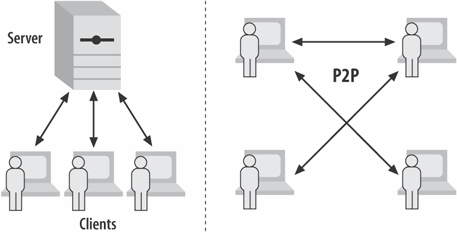
\includegraphics[scale=2]{img/p2p.png}
			\caption{Re'tea client-server vs peer-to-peer\cite{fabricdoc}}
  			\label{fig:p2p}
  		\end{center}
  		\end{figure}
Fiecare peer de'tine o copie a informa'tiilor din re'tea. Acest lucru face dificil'a modificarea abuziv'a a datelor, orice modificare fiind vizibil'a pentru ceilal'ti participan'ti.   
\subsection{Func'tii de hash 'si criptografie}
	O func'tie de hash reprezint'a o metoda unidirec'tional'a de mapare a unui 'sir de caractere de lungime arbitrar'a la un 'sir de caractere cu lungime fix'a. Propriet'a'tile necesare pentru o func'tie de hash sunt:
	\begin{itemize}
		\item \textbf{Calcul rapid}: efortul computa'tional pentru calcularea rezultatului trebuie s'a fie mic indiferent de 'sirul de intrare.
		\item \textbf{Unidirectional'a}: ob'tinerea 'sirului original din hash nefezabil'a
		\item \textbf{Determinist'a}: rezultatul pentru un anumit 'sir de intrare este acela'si indiferent de c\^ate ori este calculat. 
		\item \textbf{Rezistent'a la coliziuni}: oricare ar fi 'sirurile de intrare a,b func'tia de hash h(a) = h(b) doar dac'a a = b. Cu alte cuvinte un 'sir de intrare produce 'intotdeauna un rezultat unic.
		\item \textbf{Schimb'arile mici din 'sirul de intrare produc schimb'ari majore 'in rezultatul func'tiei de hash}.
\end{itemize}		
	 Printre algoritmii de hash folosi'ti de diferitele implement'ari ale tehnologiei blockchain se num'ar'a SHA256(Bitcoin)\cite{bitcoin} sau Keccak-256(Ethereum)\cite{eth-yellow}. Aceste func'tii sunt folosite 'si 'in cadrul mecanismelor  pentru stabilirea consensului.
	 
	 
		Pentru controlarea accesului 'in re'teaua blockchain este folosit'a metoda de criptografie cu cheie public'a. Aceasta presupune folosirea unei perechi de chei format'a dintr-o cheie privat'a 'si o cheie public'a, derivat'a din cheia privat'a. Partea public'a a cheii poate fi folosit'a pentru criptarea datelor. Datele criptate pot fi decriptate doar cu ajutorul p'ar'tii private a cheii\cite{crypto}. 
		\subsection{Mecanism de consens}
		O proprietate important'a a unei re'tele blockchain este lipsa unei autorit'a'ti centrale care sa valideze tranzac'tiile efectuate de participan'ti. Din aceast'a cauz'a apare nevoia existen'tei unor mecanisme responsabile de rezolvarea conflictelor care apar 'in cadrul re'telei 'intre 'inregistr'arile de'tinute de participan'tii din re'tea. Algorimii de consens cei mai folosi'ti sunt: Proof of Work(PoW) 'si Bizantine Fault Tolerance(BFT).
	
		PoW este algoritmul aflat 'in spatele unor monede virtuale precum Bitcoin 'si Ethereum. Algoritmul este conceput sub forma unei competi'tii 'in care participan'tii din re'tea 'i'si folosesc puterea de calcul pentru rezolvarea unei probleme\cite{pow}. Primul participant care rezolv'a problema prime'ste dreptul de a crea urm'atorul bloc din structura de date al'aturi de o anumit'a recompens'a. Rezolvarea problemei presupune efort masiv de calcul\cite{energy-bit} 'si din acest motiv este folosit'a drept masur'a de siguran'ta. Pentru a modifica intr'arile deja salvate 'in blockchain un atacator are nevoie de mai mult de 50\% din puterea de calcul a 'intregii retele, un astfel de atac fiind nefezabil. 'In acest mod este asigurat'a corectitudinea informa'tiilor, 'insa metoda folosit'a este ineficient'a.
		
		BFT asigur'a ajungerea la consens 'in cazul 'in care doar o parte din patricipan'ti sunt atacatori. Un algoritm pentru problema  cunoscut'a sub numele de "Problema generalilor bizantini"\cite{generals} a fost implementat 'in anul 1999 de Miguel Castro si Barbara Liskov sub numele de Practical Bizantine Fault Tolerance(PBFT)\cite{pbft}. Algoritmul 'incearca ajungerea la un consens 'in cadrul sistemului, p'astr'and 'in acela'si timp o laten'ta sc'azut'a 'si eficien't'a ridicat'a. Pa'sii algoritmului sunt urm'atorii:
		\begin{itemize}
			\item Un client trimite o cerere 
			\item Cererea este transmis'a celorlal'ti clien'ti
			\item Ceilal'ti clien'ti execut'a cererea 'si transmit r'aspunsul clientului care a ini'tiat cererea
			\item Clientul a'steapt'a pan'a c'and prime'ste F + 1 r'aspunsuri identice, unde F este num'arul maxim de noduri mali'tioase tolerate
			
		\end{itemize}
		Condi'tia pentru func'tionarea corect'a a sistemului este ca num'arul de noduri mali'tioase din sistem s'a fie mai mic dec'at 1/3 din num'arul total de noduri din sistem.
		
		O compara'tie la nivel 'inalt a celor dou'a mecanisme de stabilire a consensului este prezentat'a in tabelul \ref{table1}. Tabelul prezint'a o comparatie a celor doi algoritmi lu'and 'in considerare unele propriet'a'ti importante ale unei re'tele blockchain: identitatea nodurilor, performan'ta, scalabilitatea, rezisten'ta la atacuri sau puterea consumat'a.
		
	

\begin{table}[H]
\caption{Compara'tie la nivel 'inalt: PoW vs BFT}
\centering
\begin{tabular}{|p{5cm}|p{5cm}|p{5cm}|}      
\hline\hline                        
 & Proof of Work & Bizantine Fault Tolerance \\ [0.5ex]  
\hline                             
Managementul identit'a'tii nodurilor & deschis, decentralizat & fiecare nod trebuie s'a cunoasc'a inform'atii despre celelalte noduri\\ 
\hline  
Scalabilitate & excelent'a & limitat'a \\              
\hline 
Performan'ta(throuput) & limitat'a & excelent'a(mii de tranzac'tii/sec	\\
\hline 
Performan'ta(laten'ta) & laten'ta crescut'a & excelent'a(similar'a cu cea indusa de re'tea) \\
\hline 
Putere consumat'a & Ridicat'a(PoW necesit'a putere de calcul ridicat'a) & Scazut'a \\
\hline 
Num'ar total de atacatori tolera'ti & 25\% din puterea de calcul  & 33\% din num'arul de noduri care voteaz'a\\[1ex]
           
\hline                              
\end{tabular}
\label{table1} 
\end{table}

Se poate observa faptul ca algoritmii reprezint'a dou'a abord'ari diferite 'in cadrul unei re'tele blockchain. PoW pune accent pe scalabilitate dar prezint'a o performan't'a sc'azut'a 'in timp ce BFT asigur'a performan'ta ridicat'a dar cu o scalabilitate redus'a. Decizia 'in ce prive'ste tipul de algoritm folosit depinde de nevoia sistemelor implementate.
	\subsection{Smart contract}
	Un smart contract reprezint'a "un set de promisiuni 'in format digital 'in care p'artile implicate ac'tioneaz'a conform acestor promisiuni"\cite{sc}. Altfel spus aceste contracte sunt o reprezentare digital'a a unor clauze contractuale, integrate 'in software pentru a media ac'tiuni prin opera'tii bazate pe reguli. Odat'a ce precondi'tiile pentru un smart contract sunt 'indeplinite 'si acesta este ini'tiat ac'tiunile din cadrul lui sunt executate, ele fiind irevocabile.
	\subsection{Implement'ari ale tehnologiei blockchain}
	Prima implementare cu succes a tehnologiei blockchain a fost realizat'a de moneda virtual'a bitcoin. Odat'a cu cre'sterea acesteia 'in popularitate au ap'arut diverse implement'ari ale acestei tehnologii, fiecare av\^and unele particularit'a'ti 'si scopuri de utilizare diferite.
	
	
	\textbf{Tipuri de implement'ari}. Exist'a 3 tipuri de implement'ari ale tehnologiei blockchain: public, privat 'si bazat pe permisiuni\cite{permiss}\cite{ppp}. Tabelul \ref{table2} prezint'a o analiz'a la nivel 'inalt a celor 3 tipuri de implement'ari. Sunt luate 'in considerare aspecte precum drepturile de acces, performan'ta, costurile implicate, avantajele 'si dezavantajele fiecarei implement'ari precum 'si num'arul de puncte de e'sec 'in cazul fiec'areia.
		
	\textbf{Blockchain public}. 'In cadrul unul blockchain public nu exist'a nevoia definirii unor  drepturi de acces. Orice entitate are drepturi de acces egale 'in cadrul re'telei 'si poate participa la procesul de validare a tranzac'tiilor. Din acest punct de vedere un blockchain public folose'ste o topologie decentralizat'a nefiind prezent'a o autoritate central'a care s'a medieze tranzac'tiile din re'tea. O astfel de implementare este folosit'a de catre monedele virtuale Bitcoin sau Ethereum. 'In cadrul acestor re'tele participan'tii efectuaz'a tranzac'tii f'ar'a a fi implicat'a o a treia entitate 'in acest proces. Pentru a se ajunge la un consens, un mecanism de tip PoW este folosit, acesta av'and un impact asupra performan'tei re'telei 'si a consumului de enegie 'si resurse\cite{energy-bit}.
	
	\textbf{Blockchain privat}. Spre deosebire de un blockchain public, cel privat folose'ste o topologie centralizat'a. Accesul la re'tea este controlat de o autoritate central'a, aceasta av\^and dreptul de a lua decizii 'si de a implementa reguli 'in cadrul re'telei. Un astfel de blockchain poate fi folosit 'in cazul 'in care este necesar'a restric'tionarea accesului publicului larg la re'tea. O astfel de re'tea se bazaz'a pe stabilirea unui nivel ridicat de 'incredere 'in autoritatea central'a responsabil'a de administrarea re'telei. Deoarece doar o singur'a entitate este responsabil'a de procesul de validare a tranzac'tiilor, apare avantajul performan'tei crescute 'in compara'tie cu un blockchain public.
	
	\textbf{Blockchain bazat pe permisiuni}. Acest'a abordare poate fi v'azut'a ca un hibrid 'intre un blockchain privat 'si unul public. Autoritatea 'in re'tea este de'tinut'a de un set de entit'a'ti care pot face parte din organiza'tii diferite. Aceste entit'a'ti stabilesc drepturile de acces la re'tea 'si particip'a la validarea tranzac'tiilor. Drepturile de acces depind de identit'a'tile participan'tilor, fiind nevoie de executarea unor smart contracts 'inainte de executarea unor tranzac'tii pentru validarea identit'a'tii participan'tilor. Hyperledger Fabric\cite{hlfv} si Corda sunt implement'ari ale unui astfel de blockchain. Ambele sunt solu'tii open-source care pot fi folosite pentru stocarea s'i partajarea datelor 'intre participan'tii re'telei. Ambele ofer'a solu'tii pentru implementarea unei re'tele distribuite pentru stocarea 'inregistr'arilor, pun\^an\^ad accent pe protejarea datelor 'si siguran'ta acestora.
	
	
\begin{table}[h]
\caption{Compara'tie la nivel 'inalt a implement'arilor tehnologiei blockchain}
\label{table2}
\resizebox{\textwidth}{!}{%
\begin{tabular}{|l|l|l|l|}
\hline
                                                          & Public                                                                                                                                                                                                             & Privat                                                                                                                                                                                    & Bazat pe permisiuni                                                                                                                                                                                                                                                   \\ \hline
Topologie re'tea                                           & decentralizat'a                                                                                                                                                                                                     & \begin{tabular}[c]{@{}l@{}}partial\\ decentralizat'a\end{tabular}                                                                                                                          & \begin{tabular}[c]{@{}l@{}}partial\\ decentralizat'a\end{tabular}                                                                                                                                                                                                      \\ \hline
Definire                                                  & \begin{tabular}[c]{@{}l@{}}Oricine are acces \\ la datele din re'tea. \\ Toate nodurile \\ particip'a la validare\end{tabular}                                                                                       & \begin{tabular}[c]{@{}l@{}}Permisiunile de acces \\ sunt controlate de o \\ singur'a entitate de \\ 'incredere din re'tea\end{tabular}                                                       & \begin{tabular}[c]{@{}l@{}}Permisiunile de acces\\ sunt controlate de un \\ num'ar prestabilit \\ de noduri cu autoritate\end{tabular}                                                                                                                                 \\ \hline
Beneficii                                                 & \begin{tabular}[c]{@{}l@{}}- Sigur, deoarece to'ti \\ participan'tii contribuie \\ la validarea tranzac'tiilor\\ - Transparent, toate \\ tranzac'tiile fiind publice\\ iar entit'a'tile implicate\\ anonime\end{tabular} & \begin{tabular}[c]{@{}l@{}}- Verificare eficient'a \\ a tranzac'tiilor de c'atre\\ autoritatea central'a\\ - Autoritatea central'a \\ decide entita'tile care \\ au acces la re'tea\end{tabular} & \begin{tabular}[c]{@{}l@{}}- Eficient, deoarece un\\ num'ar relativ mic de\\ noduri verific'a tranzac'tiile\\ - Drepturile de acces sunt \\ controlate de un set \\ predeterminat de noduri\\ - Controlul nu este de'tinut \\ de c'atre o autoritate central'a\end{tabular} \\ \hline
Provoc'ari                                                 & Eficien'ta sc'azut'a                                                                                                                                                                                                  & \begin{tabular}[c]{@{}l@{}}Controlul este de'tinut\\ de o singur'a entitate\end{tabular}                                                                                                    &                                                                                                                                                                                                                                                                       \\ \hline
Cost                                                      & sc'azut                                                                                                                                                                                                             & ridicat                                                                                                                                                                                   & mediu                                                                                                                                                                                                                                                                 \\ \hline
Performan'ta                                               & sc'azut'a                                                                                                                                                                                                            & excelent'a                                                                                                                                                                                 & ridicat'a                                                                                                                                                                                                                                                              \\ \hline
\begin{tabular}[c]{@{}l@{}}Puncte de \\ e'sec\end{tabular} & n                                                                                                                                                                                                                  & 1                                                                                                                                                                                         & * (nodurile cu autoritate)                                                                                                                                                                                                                                            \\ \hline
\end{tabular}%
}
\end{table}

Se observ'a c'a eficien'ta 'si performan'ta re'telei scad odat'a cu cre'sterea decetraliz'arii acesteia. Aceasta se datoreaz'a metodei de stabilire a consensului 'si a num'arului de entit'a'ti implicate 'in acest mecanism.
	
\subsection{Ethereum, Hyperledger Fabric, Corda}
'In continuare este prezentat'a o compara'tie 'intre principalele solu'tii disponibile pentru implementarea unei re'tele distribuite folosind tehnologia blockchain. Aceste solu'tii sunt: Ethereum, Hyperledger Fabric si Corda\cite{comp}. Tabelul \ref{table4} prezint'a o compara'tie a caracteriticilor celor 3 solu'tii:



\begin{table}[H]
\caption{Comparatie Ethereum, Hyperledger Fabric, Corda conform cu\cite{comp}}
\centering
\begin{tabular}{|p{3cm}|p{3cm}|p{3cm}|p{3cm}|}      
\hline\hline                        
Caracteristica  & Ethereum & Hyperledger Fabric & Corda \\ [0.5ex]  
\hline                             
descriere & platforma generic'a blockchain & platform'a modular'a blockchain & solu'tie distribuit'a pentru domeniul financiar\\ 
\hline  
mod de operare  & f'ar'a permisiuni, public, privat & bazat pe permisiuni, privat & bazat pe permisiuni, privat\\              
\hline 
consens & PoW & suport pentru diferite mecanisme & consens realizat de "notary nodes" \\
\hline 
smart contract  & Solidity& Go, Java& Kotlin, Java \\
\hline 
moneda virtual'a & Ether & f'ar'a,  poate fi implementat'a cu ajutorul smart contract& f'ar'a  \\[1ex]
           
\hline                              
\end{tabular}
\label{table4} 
\end{table}

Ethereum si Hyperledger Fabric sunt g\^andite pentru utilizarea 'intr-un spectru larg de cazuri de utilizare. Spre deosebire de acestea, Corda are ca utilizare principal'a domeniul financiar\cite{cordadoc}.

'In ce prive'ste mecansimul de consens Hyperledger Fabric ofer'a posibilitatea utiliz'arii a diferite mecansime de consens. Stabilirea consensului are loc la  nivelul tranzac'tiilor 'si implic'a doar par'tile care sunt responsabile de  tranzac'tie. Nodurile din re'tea de'tin roluri diferite 'in ob'tinerea consensului. Hyperledger Fabric 'imparte nodurile din sistem 'in 3 categorii: \emph{peer, orderer, client}\cite{fabricdoc}\cite{hlfv}. Nodurile de tip \emph{peer} men'tin registrul cu date 'si primesc mesaje pentru actualizarea registrului. Nodurile de tip \emph{client} reprezint'a utilizatorii re'telei 'si au capabilitatea de a invoca tranzac'tii. Comunicarea 'intre \emph{peer}-uri prin intermediul canalelor de comunicare este asigurat'a de nodurile de tip \emph{orderer}.

Corda foloseste o abordare similar'a cu Hyperledger Fabric pentru stabilirea consensului. Aceasta are loc la nivelul tranzactiilor 'si utilizeaz'a doar p'artile implicate. Consensul trebuie determinat 'intre participan'tii re'telei numi'ti \emph{notary nodes}\cite{cordadoc}, exist\^and libertatea alegerii algoritmului folosit.

Spre deosebire de cele dou'a abord'ari de mai sus, Ethereum folose'ste un mecanism PoW. Acest aspect duce la sc'aderea performan'tei procesarii tranzac'tiilor. 

Lucarea folose'ste 'in continuare platforma Hyperledger Fabric pentru implementarea sistemului. Principala motiva'tie pentru utilizarea acestei platforme este flexibilitatea oferit'a 'in implementarea cazurilor de utilizare. Spre deosebire de Corda, cu specializare pe domeniul financiar, Hyperledger Fabric 'si Ethereum pot fi aplicate 'intr-un spectu larg de domenii. Performan'ta este un alt motiv pentru alegerea platformei Hyperledger Fabric. Posibilitatea de alegere a mecanismului de consens, spre deosebire de Ethereum, duce la imbun'at'a'tirea performan'tei 'in ce prive'ste timpul de procesare a tranzac'tiilor. 

\section{Scenarii de utilizare ale tehnologiei blockchain}
Sec'tiunea curenta descrie unele scenarii de utilizare 'in anumite domenii care pot beneficia de pe urma utiliz'arii tehnologiei blockchain. Sunt prezentate aspecte ale tehnologiei blockchain care pot ajuta la imbun'at'a'tirea metodologiilor din aceste domenii.

\textbf{Determinarea identit'a'tii digitale}. 'In prezent, detaliile despre identitatea unei persoane sunt stocate de c'atre diferite institu'tii. Din acest motiv o persoan'a poate avea o serie de identit'a'ti asupra c'arora nu de'tine controlul. Apar provoc'ari 'in ce prive'ste siguran'ta datelor cu caracter personal 'si a existen'tei unui punct unic de e'sec. 

Tehnologia blockchain poate imbun'at'a'tii procedurile din acest domeniu. Prin oferirea controlului absolut asupra identit'a'tii lor, participan'tii pot alege detaliile care vor s'a le partajeze despre identitatea lor. Aceasta identitate a unui utilizator nu va fi stocat'a de o alta entitate, ci aceste entit'a'ti vor contribui doar la validarea detaliilor despre identitatea unei persoane.

\textbf{Managementul datelor financiare}. Domeniul financiar este predispus fraudelor deoarece sistemele de contabilitate sunt controlate de entit'a'tile care le folosesc. Este necesar, de asemenea un efort uman considerabil pentru medierea tranzac'tiilor 'intre sisteme incompatibile. Toate acestea determin'a costuri ridicate de mentenan'ta, efort uman 'si timp.

Utilizarea smart contracts 'in domeniul financiar poate imbun'at'a'tii timpul de procesare a tranzac'tiilor, corectitudinea datelor 'si transparen'ta acestora. Este eliminat'a nevoia existen'tei entit'a'tilor care s'a medieze tranzac'tiile 'intre anumite p'ar'ti, acestea av\^and posibilitatea de a tranzac'tiona 'in mod direct. Fraudarea datelor este mai dificil'a, sistemul de contabilitate fiind controlat de toate entit'a'tile implicate. 

\textbf{Determinarea provenien'tei bunurilor}. Determinarea originii anumitor bunuri 'intr-un lan't de aprovizionare 'intampin'a dificult'a'ti din cauza complexit'a'tii procesului de management al unui lan't de aprovizionare 'si dorin'tei de a partaja informa'tii doar cu entit'a'tile relevante(institu'tii de reglementare, vamale, etc). Din cauza dificult'a'tilor 'int\^alnite 'in determinare originii produselor riscul existen'tei fraudelor este ridicat.

Urm'arirea provenien'tei produselor poate fi imbun'at'a'tit'a prin folosirea unei re'tele blockchain pentru 'inregistrarea datelor referitoare la originea produselor. Accesul la informa'tii este simplificat, entit'a'tile din re'tea particip\^and la validarea 'si memorarea tranzac'tiilor 'in registrul de date comun. Detectarea fraudelor este imbun'at'a'tita, fiecare entitate av\^and acces la tranzac'tiile din sistem. 

\section{Tehnologia blockchain 'in studiile clinice}
Principalele provoc'ari 'intampinate 'in cadrul studiilor clinice sunt legate de protec'tia datelor cu caracter personal 'si reducerea num'arului de fraude din acest domeniu.

Tehnologia blockchain poate avea un impact global asupra cercet'arii clinice deoarece permite urm'arirea, partajarea 'si protec'tia informa'tiilor. Prin utilizarea unui sistem decentralizat folosit pentru urm'arirea activit'a'tilor din cadrul unui studiu clinic 'si a unei re'tele peer-to-peer pentru partajarea informa'tiilor sunt asigurate transparen'ta 'si protec'tia datelor personale ale pacientilor. Un sistem bazat pe aceasta tehnologie poate imbun'at'a'ti metodologiile din cercetarea clinic'a 'si protec'tia datelor cu caracter sensibil.

\subsection{Modelarea cercet'arii clinice sub forma unei re'tele de\\ afaceri}

	O \textbf{re'tea de afaceri} reprezint'a o re'tea complex'a de companii "unde scopul este de a sus'tine cerin'tele informa'tionale 'si opera'tionale ale afacerii cum ar fi cele de marketing, contabilitate ..."\cite{bndef}. Un alt aspect important al unei re'tele de afaceri este c'a aceasta nu 'inglobeaza doar afacerea 'in sine ci implic'a 'si unele entit'a'ti din exterior care sus'tin activitatea re'telei cum ar fi furnizorii sau distribuitorii. 
	
	'In cazul studiilor clinice o re'tea de afaceri poate fi format'a din participan'tii direc'ti la activita'ti(ex. centrele medicale 'in care se desfasoar'a studiile clinice), precum 'si par'tile care sus'tin activitatea studiilor clinice(ex. furnizori, institu'tii de reglementare...)
	Re'telele existente de afaceri folosesc 'in prezent metode similare pentru stocarea informa'tiilor. Entit'atile implicate tranzac'tioneaz'a 'intre ele, 'ins'a men'tin 'inregistr'ari proprii referitoare la tranzac'tiile efectuate. 'In cele mai multe cazuri o autoritate central'a 'in care toate p'artile implicate au 'incredere intermediaz'a tranzactiile 'si schimbul de informa'tii din cadrul re'telei. Conceptul descris mai sus este ilustrat in figura \ref{fig:centralised}.\\	
		\begin{figure}[H]
		\begin{center}
			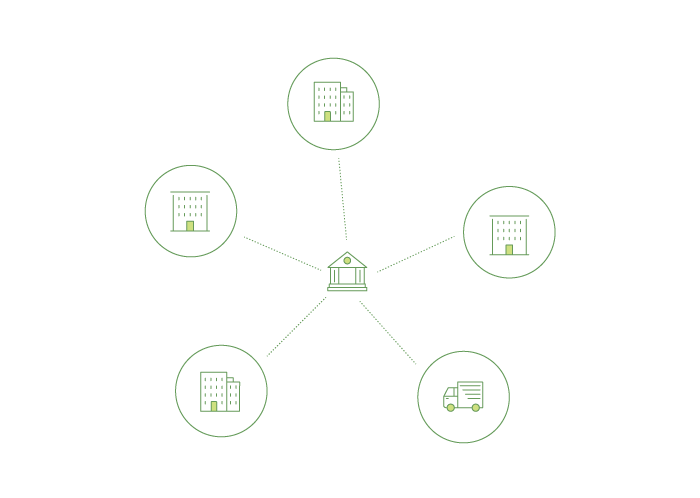
\includegraphics[scale=1.60]{img/current_network.png}
			\caption{Re'tele de afaceri centralizate\cite{fabricdoc}}
  			\label{fig:centralised}
  		\end{center}
  		\end{figure}
  		
	Aceasta metod'a prezint'a o complexitate redus'a dar produce 'in acela'si timp unele dezavantaje. Partajarea informa'tiilor este efectuat'a indirect, responsabil'a de acest lucru fiind autoritatea central'a. Din acest motiv procesul este 'incetinit, implic'and costuri suplimentare. Stabilirea corectitudinii informa'tiilor devine dificil'a 'in momentul 'in care par'tile implicate de'tin 'inregistr'ari diferite referitoare la tranzac'tii.
		Printre sistemele care folosesc o astfel de abordare se numar'a Oracle Siebel Clinical Trial Management System\cite{ctms}. Sistemul ofer'a posibilitatea cercet'atorilor de a organiza 'si colecta date 'in cadrul unui studiu clinic, fiind astfel simplificat'a activitatea acestora. Datele sunt colectate intr-o baza de date central'a . Partajarea datelor 'intre participan'ti are loc fie prin implicarea unei autorit'a'ti centrale, fie prin folosirea unor mijloace nesigure. Aceste mijloace sunt ineficiente 'si reprezint'a un risc 'in ce prive'ste protejarea datelor cu caracter sensibil.\\	

\textbf{Re'tele de afaceri decentralizate}. O alt'a abordare pentru realizarea unei re'tele de afaceri reprezint'a utilizarea unei re'tele decentralizate. O astfel de metod'a presupune folosirea unui registru comun, replicat de c'atre fiecare participant din re'teaua de afaceri. Procesul de salvare a tranzac'tiilor 'in cadrul registrului este de asemenea partajat, fiecare participant la re'tea contribuind la procesul de validare 'si memorare a tranzac'tiilor efectuate. Este eliminat'a astfel nevoia unei autorit'a'ti centrale, par'tile implicate av\^and 'incredere c'a tranzac'tiile salvate 'in registrul comun sunt valide. \\
Figura \ref{fig:decentralised} ilustreaza structura unei re'tele de afaceri decentralizate. O astfel de re'tea este similar'a cu o re'tea blockchain.
		\begin{figure}[H]
		\begin{center}
			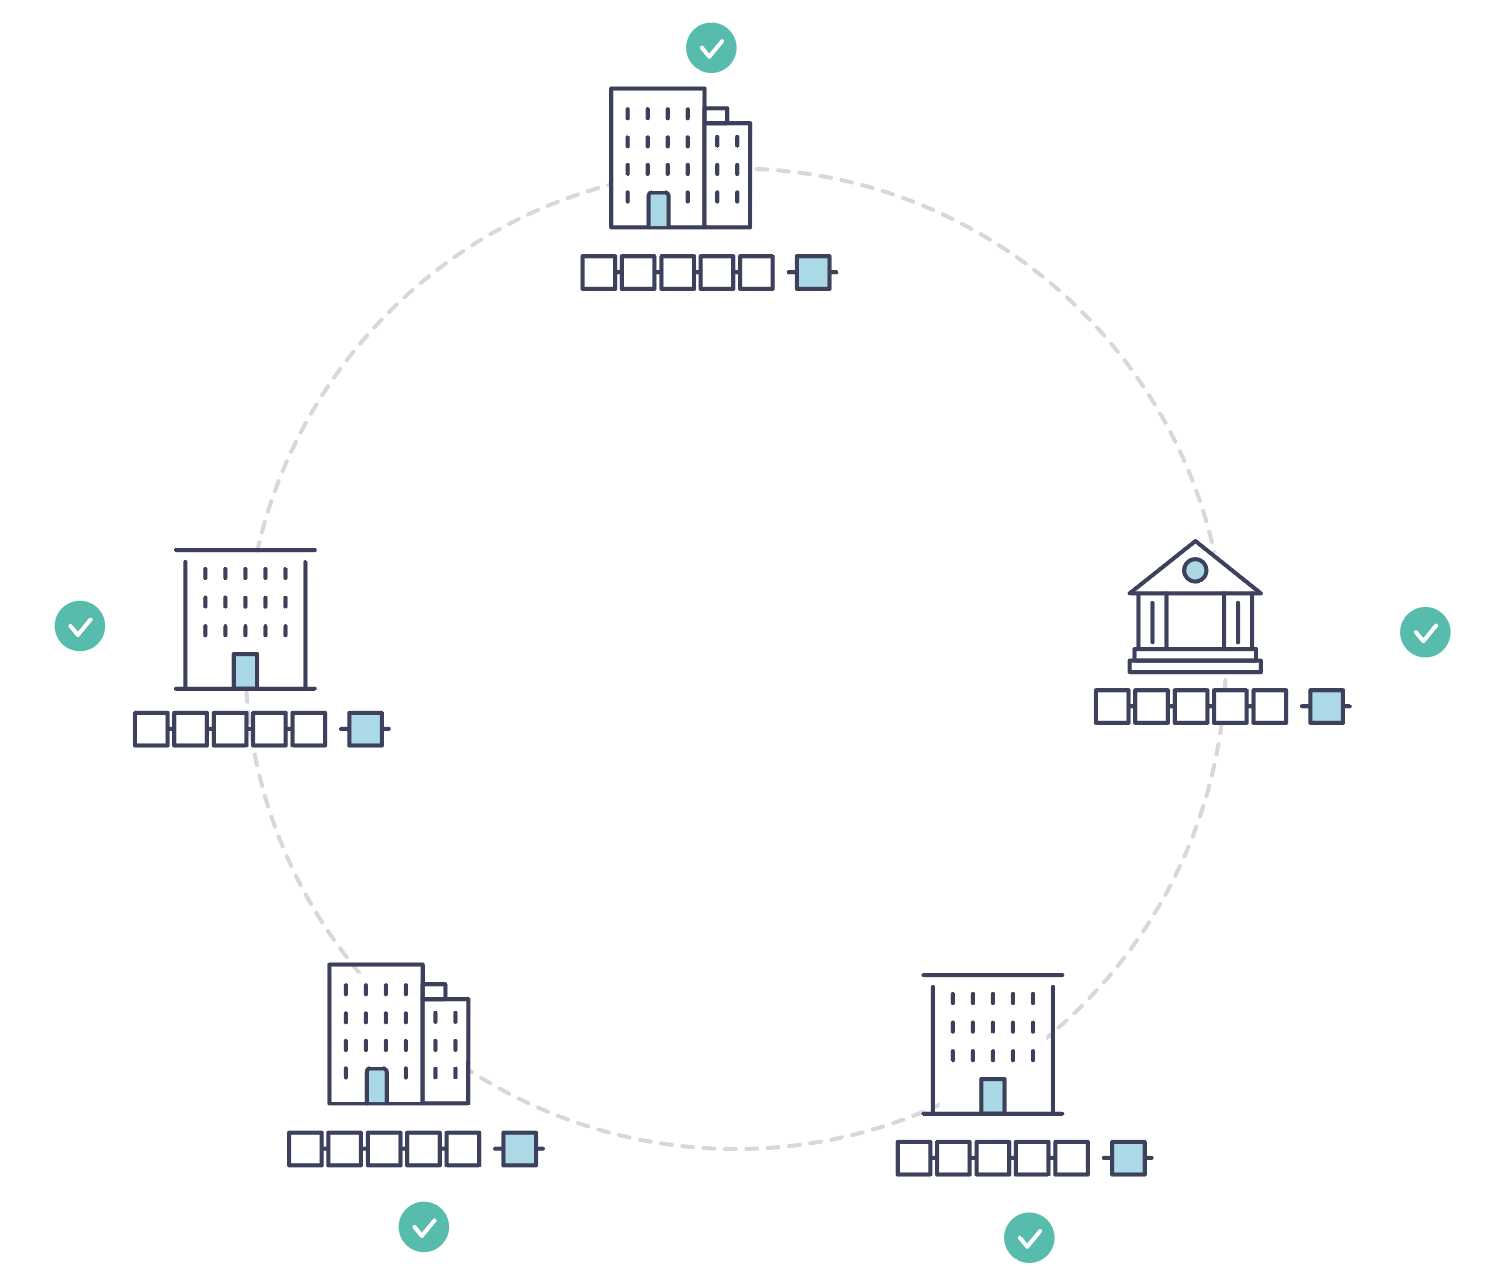
\includegraphics[scale=0.3]{img/future_net.png}
			\caption{Re'tele de afaceri decentralizate\cite{fabricdoc}}
  			\label{fig:decentralised}
  		\end{center}
  		\end{figure}
  		

\chapter{Analiz'a 'si Fundamentare Teoretic'a}
\label{ch:analysis}
Acest capitol prezint'a cerin'tele unui sistem pentru managementul studiilor clinice. Sunt prezenta'ti actorii principali ai sistemului, al'aturi de cazurile de utilizare asociate fiec'aruia. Capitolul se 'incheie printr-o prezentare a tehnologiilor folosite pentru implementarea cazurilor de utilizare, respect\^and constr\^angerile specificate de cerin'tele sistemului.

\section{Cerin'te sistem}
Sec'tiunea prezint'a o analiz'a a sistemului pentru managementul studiilor clinice. Cerin'tele unui sistem pot fi clasificate 'in cerin'te func'tionale 'si non-func'tionale. Cerin'tele func'tionale descriu comportamentul sistemului din punctul de vedere al utilizatorilor. Cerin'tele non-func'tionale descriu propriet'a'ti 'si impun constr\^angeri asupra sistemului.

\subsection{Cerinte func'tionale}
'In continuare sunt prezentate cerin'tele func'tionale 'indeplinite de modulul client al aplica'tiei. Aceste functionalit'a'ti sunt disponibile pentru utilizatorii sistemului:
\begin{enumerate}
	\item \textbf{Autentificare}: Accesul la func'tionalit'a'tile aplica'tiei este disponibil doar pentru utilizatorii autentifica'ti. Identitatea utilizatorului are o importan't'a major'a 'in cadrul retelei blockchain. 'In acest mod este asigurat'a posibilitatea  urm'ariri activit'a'tii participan'tilor 'si salvarea unui istoric a tuturor opera'tiilor efectuate de ace'stia. 
	\item \textbf{Management identitate}: Utilizatorii autentifica'ti au nevoie de o identitate emis'a de organiza'tia din care fac parte pentru a putea accesa re'teaua. Cu ajutorul acesteia utilizatorii sunt identifica'ti 'in re'teaua blockchain 'si supu'si regulilor de acces la resurse definite 'in sistem. Identitatea unui participant poate fi revocat'a, acesta pierz\^and accesul la serviciile oferite de sistem.
	\item \textbf{Management studii clinice}: Utilizatorii au posibilitatea de a crea un nou studiu clinic folosind interfa'ta utilizator dup'a introducerea informa'tiilor necesare.  Utilizatorii autentifica'ti care au drepturile de acces necesare pot accesa informa'tiile despre un studiu clinic 'si datele legate de activitatea desf'a'surat'a 'in cadrul acestora.
	\item \textbf{'Inrolare pacien'ti}: Posibilitatea de a asocia un pacient la un studiu clinic.
	\item \textbf{Colectare date}: Cercet'atorii pot defini 'in cadrul unui studiu clinic formulare de colectare a datelor de la pacien'ti. Aceste formulare ofer'a cercet'atorului flexibilitatea de a defini c'ampuri de text 'si 'intrebari cu variante de r'aspuns relevante pentru studiul clinic. Folosind formularele definite, cercet'atorii au posibilitatea de a colecta date de la un anumit pacient.
	\item \textbf{Drepturi de acces}: Permite administratorilor sistemului s'a defineasc'a drepturile de acces la resursele 'si serviciile oferite de aplica'tie.
	\item \textbf{Gestionare fi'siere}: Utilizatorii care de'tin drepturile necesare pot salva 'in sistem fi'siere de protocol 'si contracte de sponsorizare. Protocolul unui studiu clinic descrie modul de desf'a'surare al acestuia. Utilizatorii care de'tin drepturile de acces necesare pot 'inc'arca un fi'sier de protocol 'si 'il pot desc'arca prin intermediul interfe'tei utilizator.
	\item \textbf{Istoric activit'a'ti}: Sistemul colecteaz'a 'in mod automat un istoric 'in timp al opera'tiilor efectuate de utilizatori. 
\end{enumerate}

\subsection{Cerin'te non-func'tionale}
\begin{enumerate}
\item \textbf{Utilizabilitatea}. Procesele din cadrul unui studiu clinic au o complexitate ridicat'a. Din acest motiv sistemul are nevoie de o interfa't'a utilizator intuitiv'a, care s'a permit'a cercetatorilor s'a 'i'si desf'a'soare activitatea rapid. Un alt aspect important este correctitudinea informa'tiilor care poate fi imbun'at'a'tit'a prin valid'ari 'si mesaje de eroare.
\item \textbf{Securitatea}. Protec'tia datelor cu caracter sensibil are o importan't'a majora 'in studiile clinice. Accesul pentru citirea 'si scrierea datelor este oferit doar utilizatorilor autentifica'ti. 'In plus, accesul la resurse este controlat de listele de acces care definesc reguli de scriere s'i citire.
\item \textbf{Fiablitate}. Timpul i'n care serviciile oferite de sistem sunt indisponibile trebuie s'a fie minim. Acest lucru poate fi asigurat prin replicarea nodurilor din re'teaua blockchain.
\item \textbf{Performan'ta}. Performan'ta sistemului este masurat'a folosind mijloace specifice tehnologiei utilizate. Aceasa poate fi m'asurat'a 'in num'arul de tranzac'tii/secund'a sau resursele de sistem consumate.
\item \textbf{Compatibilitate}. Cerin'ta non-func'tional'a care specific'a posibilitatea de utilizare a sistemului din platforme multiple. 'In cazul sistemului de management a studiilor clinice este posibil accesul utilizatorilor din orice browser modern, mobil sau desktop. 
\end{enumerate}

\section{Cazuri de utilizare}
Sec'tiunea descrie cazurile de utilizare ale aplica'tiei analiz'and actorii implica'ti 'in realizarea acestora. Sistemul pentru managementul studiilor clinice are definite 4 tipuri principale de utilizatori: administrator, cercet'ator, agent de reglementare 'si sponsor.
%\begin{table}[H]
%\centering
%\caption{Asociere func'tionalit'a'ti - cazuri de utilizare - actori}
%\label{uc-table}
\begin{longtable}{|p{5cm}|p{5.3cm}|p{5.1cm}|}
\caption{Asociere func'tionalit'a'ti - cazuri de utilizare}
\label{uc-table}
\endfirsthead
\endhead
\hline
\hline
Func'tionalitate          & Cazuri de utilizare                        & Actori                                                 \\ \hline
Autentificare            & Autentificare utilizator                   & Cercet'ator, Agent Reglementare, Sponsor, Administrator \\ \cline{2-3} 
                         & Mapare identitate la contul utilizatorului & Cercet'ator, Agent Reglementare, Sponsor                \\ \hline
Management identitate    & Emitere identitate                         & Administrator                                          \\ \cline{2-3} 
                         & Revocare identitate                        & Administrator                                          \\ \hline
Management studiu clinic & Creare studiu clinic                       & Cercet'ator                                             \\ \cline{2-3} 
                         & Vizualizare studiu clinic                  & Cercet'ator, Agent Reglementare, Sponsor                \\ \cline{2-3} 
                         & C'autare studii clinice                     & Cercet'ator, Agent Reglementare, Sponsor                \\ \cline{2-3} 
                         & Modificare studiu clinic                   & Cercet'ator                                             \\ \hline
'Inrolare pacien'ti        & Creare pacient                             & Cercet'ator, Administrator                              \\ \cline{2-3} 
                         & C'autare pacient                            & Cercet'ator, Administrator                              \\ \cline{2-3} 
                         & 'Inrolare pacient 'in studiu clinic          & Cercetator                                             \\ \hline
Colectare date           & Creare formular personalizat               & Cercet'ator                                             \\ \cline{2-3} 
                         & Vizualizare formulare                      & Cercet'ator, Agent Reglementare                         \\ \cline{2-3} 
                         & Completare formular                        & Cercet'ator                                             \\ \cline{2-3} 
                         & Vizualizare date colectate                 & Cercet'ator, Agent Reglementare, Sponsor                \\ \hline
Drepturi de acces        & Asignare cercet'ator la studiu clinic       & Cercet'ator                                             \\ \cline{2-3} 
                         & Asignare agent reglementare                & Administrator                                          \\ \hline
Gestionare fi'siere       & Ad'augare fi'sier                            & Cercet'ator, Sponsor                                    \\ \cline{2-3} 
                         & Desc'arcare fi'sier                          & Cercet'ator, Sponsor                                    \\ \hline
Istoric activit'a'ti       & Creare istoric                             & Sistem                                                 \\ \hline
                         & Vizualizare istoric                        & Cercet'ator, Agent Reglementare, Sponsor                \\ \cline{2-3} 
                         & Filtrare istoric                           & Cercet'ator, Agent Reglementare, Sponsor                \\ \hline
\end{longtable}
%\end{table}

 Aceste 3 tipuri de utilizatori apar'tin unor organiza'tii diferite din re'teaua blockchain. Tabelul \ref{uc-table} prezint'a o asociere 'inte functionalit'a'tile sistemului, cazurile de utilizare 'si utilizatorii care particip'a la realizarea acestora.


\subsection{Cercetator} Utilizatorul apar'tine organiza'tiilor din domeniul medical 'in cadrul re'telei blockchain. Responsabilitatea sa principal'a este managementul activit'a'tilor din cadrul unui studiu clinic. 'In figura \ref{fig:ucc} sunt prezentate cazurile de utilizare asociate utilizatorului.

	\begin{figure}[H]
		\begin{center}
			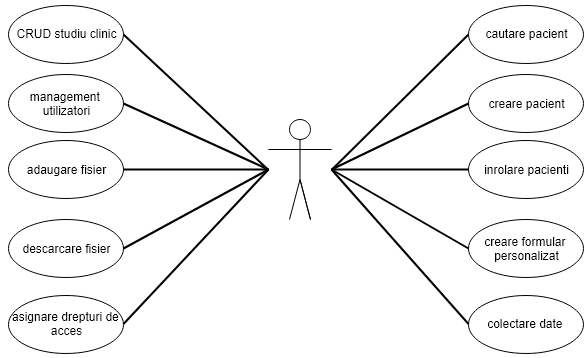
\includegraphics[scale=0.65]{img/uc_cerc.PNG}
			\caption{Cazuri de utilizare cercetator}
  			\label{fig:ucc}
  		\end{center}
  	\end{figure}
  		
 
 

\subsection{Agent de reglementare} Utilizatorul apar'tine intitu'tiilor care se ocup'a de aplicarea regulilor asupra unui studiu clinic. Aces'tia supervizeaz'a acivit'a'tile care au loc 'in cadrul unui studiu clinic cu scopul de a g'asi eventualele nereguli. Figura \ref{fig:ucr} prezint'a cazurile de utilizare 'si responsabilit'a'tile asociate agentului de reglementare.

	\begin{figure}[H]
		\begin{center}
			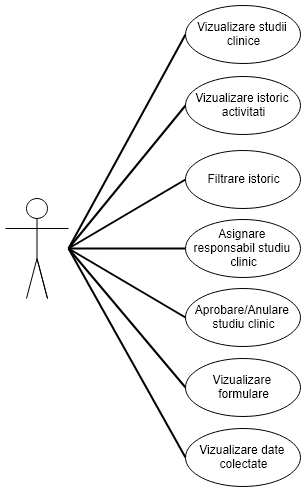
\includegraphics[scale=0.56]{img/uc_reg.PNG}
			\caption{Cazuri de utilizare agent de reglementare}
  			\label{fig:ucr}
  		\end{center}
  	\end{figure}

\subsection{Sponsor} 
    Interesat de rezultatele studiilor clinice finan'tate. Dore'ste s'a poat'a vizualiza rezultatele ob'tinute 'in timpul unui studiu clinic. Particip'a la 'incheierea contractelor de sponsorizare cu institu'tiile responsabile de organizarea studiilor clinice. 'In figura \ref{fig:ucs} sunt reprezentate cazurile de utilizare asociate utilizatorului de tip sponsor.

	\begin{figure}[H]
		\begin{center}
			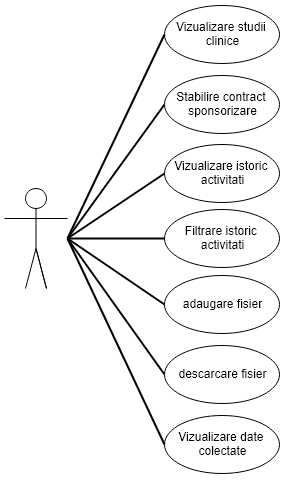
\includegraphics[scale=0.57]{img/uc_spon.PNG}
			\caption{Cazuri de utilizare sponsor}
  			\label{fig:ucs}
  		\end{center}
  	\end{figure}


\subsection{Descrierea cazurilor de utilizare}
  		
 \subsubsection{Caz de utilizare 1 - Autentificare}
 Este prezentat'a 'in continuare o descriere a mecanismului de autentificare a utilizatorilor 'in sistem. Aceasta descriere con'tine scenariul principal de succes al'aturi de extensiile cazului de utilizare\\
\textbf{Numele cazului de utilizare:} Autentificare utilizator\\
\textbf{Actor principal:} Utilizator al sistemului\\
\textbf{Stakeholders:}
\begin{itemize}
    \item Utilizatorul: dore'ste sa acceseze serviciile oferite de sistem
    \item Administrator: dore'ste ca doar utilizatorii cu identit'a'ti emise s'a poata accesa sistemul
\end{itemize}
\textbf{Precondi'tii:} f'ar'a\\
\textbf{Postcondi'tii:} sistemul determin'a identitatea utilizatorului, o afi'seaza 'si ofera acces la serviciile sistemului\\
\textbf{Scenariu de succes:} 
\begin{enumerate}
     \item Utilizatorul selecteaz'a op'tiunea de autentificare
     \item Aplica'tia redirec'tioneaz'a utilizatorul spre sistemul extern de autentificare
     \item Utilizatorul introduce creden'tialele de acces
     \item Sistemul extern furnizeaz'a un token de autentificare
     \item  Aplica'tia afi'seaz'a identitatea utilizatorului 'si 'ii permite accesul
\end{enumerate}
\textbf{Scenarii alternative:}
\begin{itemize}
    \item 3a. Utilizatorul introduce creden'tiale gre'site:
        \begin{enumerate}
            \item Sistemul extern afi'seaza un mesaj de eroare 'si solicita creden'tialele
        \end{enumerate}
    \item 3b. Utilizatorul este la prima autentificare 'in sistem
        \begin{enumerate}
            \item Sistemul extern cere permisiunea pentru autorizarea aplica'tiei
            \item Utilizatorul selecteaz'a optiunea de autorizare acces
            \item Sistemul extern furnizeaz'a un token de autentificare
        \end{enumerate}
    \item 5a. Utilizatorul nu are o identitate definit'a 'in re'tea
        \begin{enumerate}
            \item Aplica'tia cere un cod de inrolare i'n sistem
            \item Utilizatorul introduce codul furnizat de administra'tia organiza'tiei din care face parte
            \item Aplica'tia salveaz'a o asociere 'intre identitatea utilizatorului 'si contul acestuia
        \end{enumerate}
\end{itemize}

\subsubsection{Caz de utilizare 2 - Creare formular personalizat}
Cercet'atorii au la dispozitie o func'tionalitate prin care pot defini un formular 'in func'tie de nevoile 'int\^alnite 'in cadrul unui studiu clinic. 'In continuare sunt descri'si actorii implica'ti, al'aturi de pa'sii care trebuie urma'ti 'in definirea unui formular.
\textbf{Numele cazului de utilizare:} Creare formular personalizat\\
\textbf{Actor principal:} Cercet'ator\\
\textbf{Stakeholders:}
\begin{itemize}
    \item Cercet'ator: doreste ca sistemul s'a ii ofere flexibilitatea de a defini c\^ampurile de care are nevoie 'intr-un formular
    \item Agent de reglementare: interesat de corectitudinea datelor colectate. Dore'ste sa aib'a acces la informa'tii
    \item Sponsor: interesat de structura formularului de colectare a datelor
\end{itemize}
\textbf{Precondi'tii:} Utilizator autentificat, cu drepturi de citire 'si scriere asupra unui studiu clinic\\
\textbf{Postconditii:} Formularul definit este salvat 'in baza de date 'si poate fi vizualizat 'in orice moment\\
\textbf{Scenariu de succes:} 
\begin{enumerate}
    \item Utilizatorul selecteaz'a op'tiunea de creare a unui formular nou
    \item Utilizatorul introduce numele formularului
    \item Utilizatorul selecteaza tipul de c\^amp pe care dore'ste s'a 'il creeze: text field, choice sau selection
    \item Sistemul cere definirea c\^ampului
    \item Utilizatorul introduce numele 'si, dup'a caz, variantele de r'aspuns pentru c\^ampul respectiv
    \item Utilizatorul repet'a pa'sii 3-5 p\^an'a c\^and confirm'a salvarea formularului
    \item Sistemul afi'seaza un mesaj de confirmare a salvarii
\end{enumerate}
\textbf{Scenarii alternative:}
\begin{itemize}
    \item 1-5a. Utilizatorul anuleaz'a crearea formularului
        \begin{enumerate}
            \item Sistemul inl'atur'a informa'tiile introduse de utilizator
        \end{enumerate}
    \item 2a. Utilizatorul nu introduce un nume pentru formular
        \begin{enumerate}
            \item Sistemul notific'a utilizatorul printr-un mesaj de eroare
        \end{enumerate}
    \item 5a. Utilizatorul nu introduce datele necesare sau introduce date gre'site
      \begin{enumerate}
            \item Sistemul notific'a utilizatorul printr-un mesaj de eroare
            \end{enumerate}
\end{itemize}

\subsubsection{Caz de utilizare 3 - Ad'augare fi'sier}
\textbf{Numele cazului de utilizare:} Ad'augare fi'sier\\
\textbf{Actor principal:} Cercet'ator, Sponsor\\
\textbf{Stakeholders:}
\begin{itemize}
    \item Cercet'ator: dore'ste o modalitate de stocare 'si partajare a fi'sierului de protocol cu p'ar'tile interesate
    \item Sponsor: interesat de anumite fi'siere stocate. Dore'ste s'a poat'a avea acces la acestea
    \item Agent reglementare: dore'ste s'a aiba posibilitatea de a verifica fi'sierele inc'arcate pentru a putea aplica regulile 'in vigoare
\end{itemize}
\textbf{Precondi'tii:} Utilizator autentificat, cu drepturi de citire 'si scriere asupra unui studiu clinic\\
\textbf{Postcondi'tii:} Sistemul salveaz'a fi'sierul, acesta fiind disponibil pentru desc'arcare pentru utilizatorii cu drepturi de acces \\
\textbf{Scenariu de succes:} 
\begin{enumerate}
    \item Utilizatorul selecteaz'a op'tiunea de 'incarcare a unui fi'sier nou
    \item Sistemul cere calea spre fi'sierul dorit
    \item Utilizatorul selecteaz'a fi'sierul 'si confirm'a selec'tia
    \item Sistemul afi'seaz'a informa'tii despre fi'sier
    \item Utilizatorul selecteaz'a op'tiunea de confirmare a salv'arii
\end{enumerate}
\textbf{Scenarii alternative:}
\begin{itemize}
    \item 3a. Utilizatorul selecteaz'a un tip invalid de fi'sier
        \begin{enumerate}
            \item Sistemul notific'a utilizatorul printr-o eroare
            \item Sistemul revine la pasul 2.
        \end{enumerate}
    \item 4a. Sistemul nu poate g'asi fi'sierul selectat de utilizator
        \begin{enumerate}
            \item Sistemul notific'a utilizatorul printr-o eroare
            \item Sistemul revine la pasul 2.
        \end{enumerate}
    \item 5a. Salvarea fi'sierului e'sueaz'a
        \begin{enumerate}
            \item Sistemul notific'a utilizatorul printr-o eroare
            \item Sistemul revine la starea ini'tial'a
        \end{enumerate}
    
\end{itemize}
\section{Tehnologii utilizate}
'In continuare sunt descrise tehnologiile, resursele 'si serviicile necesare pentru implementarea sistemului 'si respectarea cerin'telor func'tionale 'si non-func'tionale ale acestuia.
\subsection{Hyperledger Fabric}\label{section:fab}
Hyperledger Fabric este platforma folosit'a pentru implementarea re'telei de afaceri pentru studii clinice. Reprezint'a un registru distribuit cu o arhitectur'a modular'a care permite participan'tilor s'a gestioneze tranzac'tii 'in sistem cu ajutorul smart contracts. Framework-ul permite implementarea de componente modulare precum algoritmi de consens. 

'In compara'tie cu Bitcoin, Hyperledger Fabric ofer'a posibilitatea implement'arii unui blockchain privat sau bazat pe permisiuni de acces. Acest lucru este realizat de serviciul de furnizare identit'a'ti folosit pentru a valida 'si autentifica participan'tii din re'tea. 'In continuare sunt prezentate caracteristicile care au dus la alegerea framework-ului pentru implementarea sistemului.

\textbf{Registru distribuit}. Fiecare participant din re'tea de'tine o copie a registrului. Acesta este format din dou'a componente: starea curent'a a re'telei 'si istoricul tranzac'tiilor. Starea curent'a a re'telei poate fi interpretat'a drept baza de date a registrului la un anumit punct din timp. Baza de date stocheaz'a structurile de date din re'tea sub forma unor perechi cheie-valoare. Istoricul tranzac'tiilor con'tine tranzac'tiile care au realizat modific'ari asupra st'arii curente a re'telei. 

\textbf{Smart contracts}. Hyperledger Fabric folose'ste un limbaj propriu pentru smart contracts numit chaincode. Acesta este responsabil de modelarea structurilor de date din re'tea 'si de gestionarea logicii re'telei.

\textbf{Protectia datelor}. Framework-ul separ'a tranzac'tiile din sistem 'in functie de participan'tii care au acces la acestea. Sunt furnizate canale pentru efectuarea tranzac'tiilor care permit accesul doar participan'tilor care au acest drept.

\textbf{Mecanism de consens}. Este permis'a configurarea mai multor algoritmi de consens. Hyperledger Fabric asigur'a suport pentru diferite implement'ari: Solo, Kafka, Simple Bizantine Fault Tolerant, etc\cite{fabricdoc}. Aceast'a caracteristic'a ofer'a un avantaj major din punct de vedere al performan'tei 'in compara'tie cu mecanismul PoW folosit de Bitcoin sau Ethereum.

\subsection{Hyperledger Composer}\label{sssec:num1}
Hyperledger Composer\footnote{https://hyperledger.github.io/composer/latest/} este un framework care are ca scop simplificarea implement'arii cazurilor de utilizare 'si a logicii unei aplica'tii care ruleaz'a 'in cadrul platformei Hyperledger Fabric.

Figura \ref{fig:comp} prezint'a artefactele necesare pentru implementarea unei re'tele blochain cu ajutorul Hyperledger Composer. Un fi'sier cu extensia .bna(\textbf{Business Network Archive}) este rezultatul implement'arii cazurilor de utilizare 'si al logicii aplica'tiei.

\textbf{Model File}. Folosit pentru modelarea layer-ului de date al aplica'tiei. Hyperledger Composer utilizeaz'a un limbaj orientat-obiect propriu pentru definirea resurselor din re'tea. Tabelul \ref{table3} prezint'a resursele care pot fi definite folosind limbajul de modelare al Hyperledger Composer al'aturi de defini'tii 'si exemple pentru acestea.

\begin{table}[H]
\caption{Defini'tii ale resurselor disponibile 'in limbajul de modelare}
\centering
\begin{tabular}{|p{2cm}|p{5cm}|p{5cm}|}      
\hline\hline                        
Denumire & Defini'tie & Exemplu \\ [0.5ex]   % inserare tabel
%heading
\hline                             
Asset & bunuri tangibile sau intangibile, servicii, etc & studiu clinic\\ 
\hline  
Participant & Actor din sistem & cercet'ator, agent de reglementare\\              
\hline 
Tranzac'tie  & Logica pentru interac'tiunile 'intre participan'ti & creare studiu clinic   \\
\hline
Concept & clase abstracte, nu pot fi stocate direct ci doar ca parte a unui asset, participant sau tranzac'tie & adresa \\
[1ex]
           
\hline                              
\end{tabular}
\label{table3} 
\end{table}


Limbajul permite crearea unor rela'tii 'intre obiectele definite. O rela'tie este reprezentat'a prin \emph{namespace}-ul unui tip, \emph{numele} tipului referit 'si \emph{identificatorul} unei instan'te din acest tip. Aceste rela'tii pot fi folosite pentru filtrarea resurselor cu ajutorul interog'arilor.

\textbf{Script File}. Acest artefact define'ste logica executat'a 'in cadrul tranzactiilor din sistem. Aceasta logic'a este descris'a folosind limbajul JavaScript. Parametrul de intrare al unei tranzac'tii este definit 'in fi'sierul de model al aplica'tiei. Tranzac'tiile definite 'in acest fi'sier pot emite evenimente prin care poate fi notificat'a interfa'ta utilizator de unele schimb'ari efectuate asupra resurselor.

\textbf{Acces control rules}. Con'tine regulile de scriere 'si citire asupra resurselor din sistem. Aceste reguli sunt aplicate asupra participan'tilor din sistem 'si pot asigura protec'tia datelor cu caracter sensibil. Regulile sunt aplicate asupra participan'tilor 'si resurselor definite in fisierul de model.

\textbf{Query Definitions}. Reprezint'a interog'ari ale st'arii curente a re'telei similare cu interogarile din SQL. Aceste interog'ari sunt definite 'in sintaxa proprie Hyperledger Composer 'si pot fi folosie pentru a filtra informa'tiile din re'tea conform unor condi'tii.

		\begin{figure}[H]
		\begin{center}
			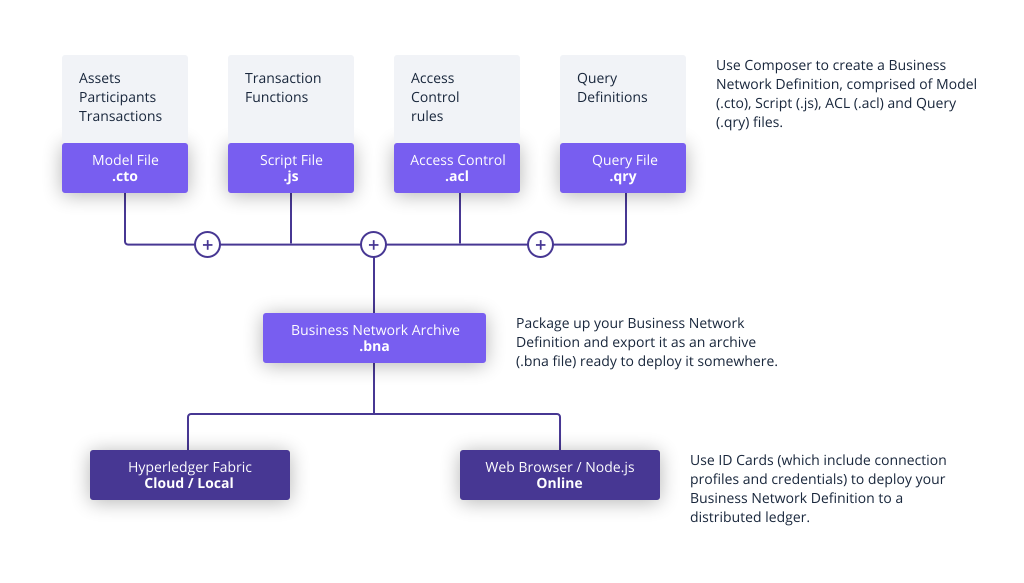
\includegraphics[scale=0.60]{img/composer.png}
			\caption{Implementarea unei re'tele blockchain uitliz\^and Hyperledger Composer}
  			\label{fig:comp}
  		\end{center}
  		\end{figure}
  		
\subsection{MongoDB}
MongoDB\footnote{https://www.mongodb.com/} este o baza de date non-rela'tional'a conceput'a de compania 10gen. Diferen'ta principala fa't'a de bazele de date rela'tionale este in stocarea informa'tiilor nu 'in tabele ci 'in fi'siere care utilizeaz'a formatul BSON(binary JSON). Aceste fi'siere sunt organizate sub forma unor colec'tii care sunt similare cu tabele din bazele de date rela'tionale. Sistemul pentru managementul studiilor clinice folose'ste aceasta baz'a de date intern
pentru a persista asocieri 'intre identit'a'tile utilizatorilor 'in re'teaua blockchain 'si conturile de utilizator ale acestora.

\subsection{Loopback}
Loopback\footnote{https://loopback.io/} este un framework Node.js care permite generarea rapida a unui server REST din diferite tipuri de surse de date. Sunt disponibili conectori pentru baze de date(SQL, MongoDB) sau pentru o surs'a de date precum Hyperledger Composer. Loopback utilizeaz'a modelul de date scris 'in Hyperledger Composer pentru a genera opera'tii CRUD pentru aplica'tie 'si puncte de acces pentru executarea tranzac'tiilor 'si a logicii acestora.

\subsection{Passport}
Passport\footnote{http://www.passportjs.org/} este un middleware pentru Node.js av\^and ca scop autentificarea cererilor. Sunt puse la dispozitie diferite stategii de autentificare folosind protocolul OAuth. Printre aceste strategii se numar'a platforme web populare cum ar fi: Google, Github, etc. Identitatea unui utilizator poate fi stocat'a fie 'in cadrul sesiunii unui browser fie 'in interiorul unui request.
\subsection{OAuth}
OAuth este un framework de autorizare care permite aplica'tiilor s'a limiteze accesul la anumite resurse doar utilizatorilor autentifica'ti, folosind servicii externe sistemului(Google, Github, etc). Sistemul de management al studiilor clinice utilizeaz'a acest protocol pentru gestionarea accesului utilizatorilor la resursele re'telei blockchain.

Protocolul OAuth define'ste 4 roluri:
\begin{enumerate}
    \item Resource owner: este utilizatorul care autorizeaz'a accesul la informa'tii legate de contul s'au
    \item Authorization  server: reprezint'a serverul care g'azduie'ste informa'tiile despre contul unui utilizator 'si care expune un API pentru autorizare
    \item Client: aplica'tia care dore'ste sa acceseze informa'tiile legate de contul unui utilizator
    \item Resource server: con'tine resursele accesibile doar utilizatorilor autentifica'ti
\end{enumerate}

	\begin{figure}[H]
		\begin{center}
			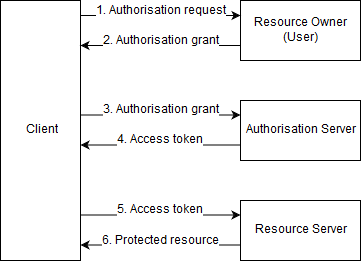
\includegraphics[scale=0.50]{img/oauth.png}
			\caption{Model abstract de func'tionare al protocolului OAuth\cite{oauth}}
  			\label{fig:oauth}
  		\end{center}
  		\end{figure}
  		
Figura \ref{fig:oauth} prezint'a modul de func'tionare al protocolului:
\begin{enumerate}
    \item Aplica'tia trimite o cerere de autorizare serverului care de'tine informa'tii despre utilizator
    \item 'In cazul 'in care utilizatorul autorizeaz'a cererea aplica'tia prime'ste acces
    \item Aplica'tia cere un token de acces prin prezentarea identit'a'tii utilizatorului 'si a confirm'arii de autorizare
    \item Serverul de autorizare returneaz'a un token de autorizare 'in cazul 'in care informa'tiile trimise de aplica'tie sunt valide
    \item Aplica'tia cere o anumit'a resursa cu acces limitat prin prezentarea token-ului de acces
    \item Serverul de resurse returneaz'a resursa cerut'a 'in cazul 'in care tokenul de acces este valid
    \end{enumerate}
    
\subsection{Docker}
    Platforma Docker\footnote{https://www.docker.com/} furnizeaz'a o solu'tie de virtualizare la nivelul sistemului de operare. Aceasta permite rularea de pachete software 'in interiorul unor \emph{containere}. Fiecare container dispune de resursele necesare pentru a asigura func'tionarea corect'a a pachetelor software. Containerele sunt izolate unele fa't'a de celelalte 'insa pot comunica prin intermediul unor canale de comunicare definite. Abordarea folosit'a de docker pentru distribuirea solu'tiilor software contribuie la simplificarea procesului de instalare al unei re'tele blockchain.
\subsection{Angular}
    Angular\footnote{https://www.angular.io/} este un framework g\^andit pentru implementarea de aplicatii web bazat pe TypeScript. Framework-ul permite implementarea de aplicatii web dinamice folosind HTML pentru reprezentarea paginilor web, dar furniz\^and posibilitatea de extindere a acestui limbaj prin implementarea de componente. 



\newpage
\thispagestyle{empty}
\mbox{}

\chapter{Proiectare de Detaliu 'si Implementare}
    'In acest capitol este prezentat'a arhitectura conceptual'a a sistemului 'si interac'tiunea dintre componentele acestuia. Sunt descrise responsabilit'a'tile fiec'arei componente al'aturi de arhitectura 'si detaliile de implementare ale acestora.
    
    \section{Arhitectura conceptual'a a sistemului}
    Principalele componente ale sistemului de management al studiilor clinice sunt mediul de rulare blockchain, serverul REST utilizat ca punct de acces 'in re'teaua blockchain 'si interfa'ta utilizator care permite participan'tilor s'a interac'tioneze cu re'teaua blockchain prin intermediul serverului REST. Arhitectura de nivel 'inalt a aplica'tiei este prezentat'a 'in figura \ref{fig:arhh}
    	\begin{figure}[H]
		\begin{center}
			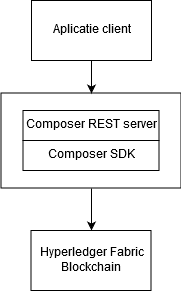
\includegraphics[scale=0.46]{img/arh_h.png}
			\caption{Arhitectura de nivel 'inalt a sistemului}
  			\label{fig:arhh}
  		\end{center}
  		\end{figure}
    
    Hyperledger Composer pune la dispozi'tie un set de tool-uri 'si SDK-uri care simplific'a interac'tiunea cu o re'tea blockchain 'si procesul de instalare al acesteia. O componenta important'a a Hyperledger Composer este framework-ul Loopback folosit 'in generarea serverului REST. Figura \ref{fig:arhc} prezint'a componentele principale ale sistemului implementat 'si interac'tiunile dintre aceste componente.
    	\begin{figure}[H]
		\begin{center}
			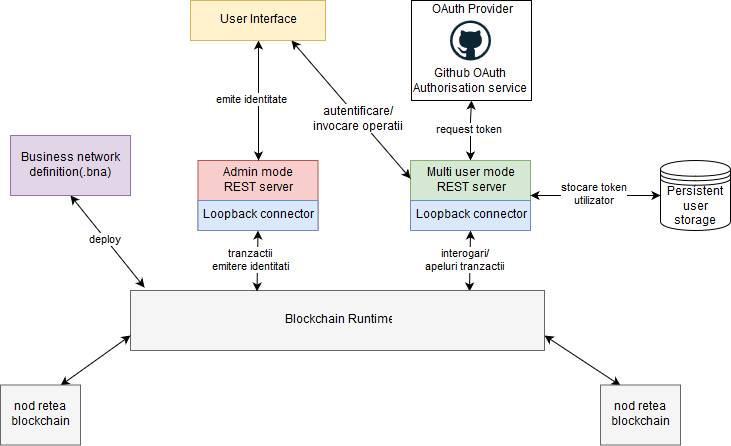
\includegraphics[scale=0.50]{img/arhc.png}
			\caption{Arhitectura conceptual'a a sistemului}
  			\label{fig:arhc}
  		\end{center}
  		\end{figure}
  Re'teaua blockchain utilizeaz'a defini'tia re'telei de afaceri (artefactul cu exensia .bna) creat cu ajutorul framework-ului Hyperledger Composer descris 'in sec'tiunea \ref{sssec:num1}. Interac'tiunea 'intre re'teaua blockchain 'si interfa'ta utilizator se realizeaz'a prin intermediul unui server REST, acesta la r\^andul lui utiliz\^and un connector Loopback pentru a accesa re'teaua. Managementul utilizatorilor se realizeaz'a de asemenea la nivelul serverului REST prin utilizarea unui serviciu extern de autentificare. O baz'a de date MongoDB asigur'a persisten'ta identit'a'tii utilizatorilor 'in sistem, 'in rela'tie cu identitatea furnizat'a de serviciul extern de autentificare.
  
  \subsection{Defini'tia re'telei de afaceri}
  
  Aceasta component'a con'tine implementarea modelului de date al aplicatiei, regulile de acces la resurse, interogarile asupra resurselor 'si logica aflat'a 'in spatele cazurilor de utilizare. 
  
  \textbf{Modelul de date al aplicatiei}. Figura \ref{fig:daig} prezint'a \emph{asset}-urile, \emph{participan'tii} 'si \emph{conceptele} principale definite 'in modelul de date al aplica'tiei. Diagrama con'tine doar elementele importante din modelul de date al aplica'tiei, cele mai pu'tin relevante fiind omise pentru p'astra complexitatea diagramei la un nivel redus. 
  
      	\begin{figure}[H]
		\begin{center}
			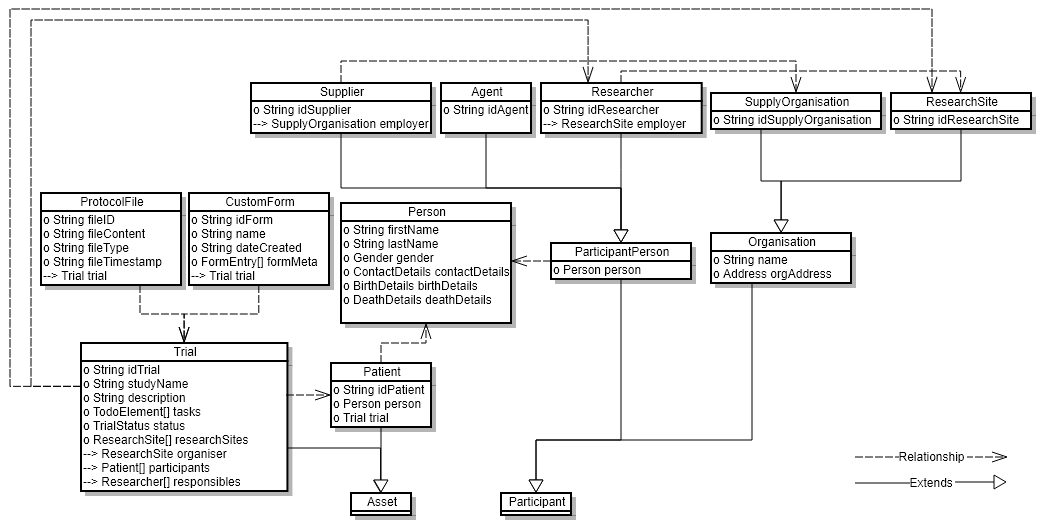
\includegraphics[scale=0.60]{img/daig.PNG}
			\caption{Modelul de date al aplica'tiei}
  			\label{fig:daig}
  		\end{center}
  		\end{figure}
  
  
  Modelarea conceptelor este realizat'a cu ajutorul limbajului orientat obiect pus la dispozi'tie de Hyperledger Composer. Figura \ref{fig:asset} prezint'a modelarea unui studiu clinic sub forma unui asset, extras din codul aplica'tiei. 
  
 	\begin{figure}[H]
		\begin{center}
			\begin{lstlisting}[style=htmlcssjs]
/** Clinic trial represented as an asset*/
asset Trial identified by idTrial{
    o String idTrial
    o String studyName
    o String description 
    o TodoElement[] tasks optional
    o TrialStatus status optional
    o ResearchSite[] researchSites optional
    --> ResearchSite organiser
    --> Patient[] participants optional
    --> Researcher[] responsibles optional
}
			\end{lstlisting}
			\caption{Studiu clinic modelat subforma unui asset}
  			\label{fig:asset}
  		\end{center}
  		\end{figure}
  
  Caracterul "o" folosit la 'inceputul unei variabile marcheaz'a o proprietate specific'a asset-ului descris. Pe l\^ang'a valori primitive\footnote{ex.: String, Boolean, Double, etc.} exist'a posibilitatea de a utiliza descrierile altor concepte 'in cadrul unui concept. Un vector de date este specificat prin utilizarea caracterelor "[]" dupa definirea tipului unei variabile\footnote{ex.: String[], ResearchSite[], etc}. O rela'tie spre un alt concept este modelat'a prin folosirea caracterelor "-->" 'inainte de definirea variabilei. 
  
  Fiecare asset este identificat 'in sistem prin intermediul unui identificator unic. Deoarece sistemul foloseste o arhitectura distribuit'a, bazat'a pe mecanisme de consens, implementarea unei functionalit'a'ti pentru generarea automat'a a identificatorilor similar cu mecanismele folosite de catre bazele de date rela'tionale este dificil'a. 'In situa'tia 'in care fiecare peer 'incearca s'a genereze urm'atorul id 'in mod concurent, pot avea loc conflicte, ceea ce ar duce la anularea unor tranzac'tii, condi'tii de cursa 'si dificult'a'ti 'in depanarea problemelor. Solu'tia la aceasta problem'a este asignarea responsabilit'a'tii de generare a unui ID aleator clientului din sistem. O astfel de abordare duce la cre'sterea eficien'tei 'si evitarea problemelor legate de concuren'ta. Un client poate folosi o func'tie simpl'a pentru generarea unui sir de caractere aleator 'si transiterea lui spre server pentru a fi utilizat ca identificator al resursei nou create. Un exemplu de func'tie care genereaz'a un 'sir de caractere aleator este prezentat 'in figura \ref{fig:rand}.
  
      	\begin{figure}[H]
		\begin{center}
				\begin{lstlisting}[style=htmlcssjs]
//generate a random id for new resources
generateID() {
    var id = "";
    for(var i = 0; i < 4; i++){
        id += Math.random().toString(36).slice(-4);
    }
    return id;
}
			\end{lstlisting}
			\caption{Generarea unui 'sir de caractere aleator 'in limbajul TypeScript}
  			\label{fig:rand}
  		\end{center}
  		\end{figure}

\textbf{Reguli de acces la resurse.} Limitarea accesului participan'tilor la resurse este o caracteristic'a necesar'a pentru protec'tia datelor cu caracter personal ale utilizatorilor din sistem. Regulile de acces 'in sistem sunt definite folosind sintaxa proprie Hyperledger Composer. Elementele principale din gramatica unei reguli de acces sunt: 
\begin{itemize}
    \item \textbf{Descriere:} O scurt'a descriere a regulii de acces folosit'a pentru o mai bun'a in'telegere a acesteia
    \item \textbf{Participant:} Specific'a tipul de participant din re'tea asupra caruia se aplic'a regula de acces 
    \item \textbf{Operatie:} Tipul de opera'tie efectuat'a de participant asupra unei resurse: CREATE, DELETE, UPDATE, READ, ANY.
    \item \textbf{Resursa:} Define'ste obiectele asupra c'arora se aplic'a regulile de acces la opera'tiile men'tionate
    \item \textbf{Transactie:} Specific'a tranzac'tia 'in cadrul c'areia sunt permise opera'tiile descrise 'in regul'a
    \item \textbf{Condi'tie:} O expresie booleana 'in limbajul JavaScript care determin'a declan'sarea unei anumite reguli
    \item \textbf{Action:} Determin'a ac'tiunea care are loc dupa declan'sarea regulii de acces. Aceasta proprietate poate avea dou'a valori: ALLOW, DENY.
\end{itemize}

Figura \ref{fig:acl} prezint'a o regul'a de acces la resursa de tip studiu clinic, aplicat'a asupra participan'tilor de tip cercet'ator. Condi'tia de declan'sare a regulii de acces este descris'a folosind limbajul JavaScript. Cu ajutorul func'tiei \emph{some} este posibil'a scanarea vectorului de participan'ti. Se poate determina astfel dac'a se permite accesul unui anumit participant la resursa respectiv'a. 'In cazul de mai jos accesul este permis doar cercet'atorilor afla'ti 'in lista de responsabili pentru un studiu clinic.

    	\begin{figure}[H]
		\begin{center}
			\begin{lstlisting}[style=htmlcssjs]

rule ResearcherTrialAccess{
    description: "Grant access to trial resources only to trial responsibles"
    participant(p): "ro.utcluj.clinictrial.base.Researcher"
    operation: READ, UPDATE
    resource(r): "ro.utcluj.clinictrial.trial.Trial"
    condition: (
        r.responsibles.some(function (responsible){
            return responsible.getIdentifier() == p.getIdentifier();
        })
    )
    action: ALLOW
}
						\end{lstlisting}
			\caption{Exemplu regul'a de acces}
  			\label{fig:acl}
  		\end{center}
  		\end{figure}


\textbf{Interog'ari.} Permit filtrarea resurselor din sistem pe baza unor criterii. Interog'arile din re'tea sunt descrise 'in sintaxa Hyperledger Composer, sintaxa similara cu cea 'int\^alnit'a 'in interog'arile SQL. O interogare este compus'a din dou'a propriet'a'ti: 
\begin{itemize}
    \item \textbf{Descriere:} Specific'a modul de func'tionare al interog'arii
    \item \textbf{Statement:} Con'tine condi'tia interog'arii folosind operatori similari cu cei din limbajul SQL(SELECT, FROM, WHERE, AND, OR, etc.)
\end{itemize}

\textbf{Tranzac'tii}. Unele cazuri de utilizare necesit'a o logic'a mai complexa dec\^at opera'tiile CRUD. 'In aceste cazuri este necesar'a implementarea unei logici de procesare adi'tionale. Acest lucru poate fi realizat prin implementarea unor tranzac'tii care descriu comportamentul cazului de utilizare. 

    	\begin{figure}[H]
		\begin{center}
		
			\begin{lstlisting}[style=htmlcssjs]
/**
 * Adds a Researcher as responsible for a clinical trial
 * @param {ro.utcluj.clinictrial.trial.AddResearcherToTrial} tx 
 * @transaction
 */
async function addResearcherToTrial(tx) {
  console.log('Adding researcher to the responsibles list...');
  //namespace for transaction
  const factory = getFactory();
  const NS_TRIAL = 'ro.utcluj.clinictrial.trial';
  const NS_BASE = 'ro.utcluj.clinictrial.base';
  let trial = tx.trial;
  let researcher = tx.researcher;
  //check for duplicates
  for (let index in trial.responsibles) {
    if (trial.responsibles[index].idResearcher == researcher.idResearcher) {
      throw new Error('Duplicate entry');
    }
  }
  //add relations
  trial.responsibles
    .push(factory
      .newRelationship(NS_BASE, 'Researcher', researcher.idResearcher));
  console.log('Updating trial ...');
  const registry = await getAssetRegistry(
                            trial.getFullyQualifiedType());
  await registry.update(trial);
}
			\end{lstlisting}
			\caption{Ad'augarea unui nou responsabil pentru un studiu clinic}
  			\label{fig:tranz}
  		\end{center}
  		\end{figure}

Comentariul unei tranzac'tii con'tine pe primul r\^and o descriere a opera'tiei efectuate de tranzac'tie. Al doilea r\^and 'incepe cu adnotarea \textbf{@param} folosit'a pentru a marca definirea parametrului tranzac'tiei. Adnotarea  \textbf{@param} este urmat'a de numele complet al resursei care declan'seaza tranzac'tia(namespace + tip) alaturi de numele parametrului folosit de tranzac'tie. Ultimul r\^and con'tine adnotarea  \textbf{@transaction} care specific'a faptul c'a func'tia trebuie interpretat'a ca fiind o tranzac'tie.
Parametru func'tiei este descris 'in modelul de date al aplica'tiei. Pentru exemplul din figura \ref{fig:tranz} descrierea parametrului tranzac'tiei 'in limbajul de modelare poate fi observat'a 'in figura \ref{fig:par}. 'In acest exemplu pentru crearea unei rela'tii 'intre un studiu clinic 'si un cercet'ator, o tranzac'tie are nevoie de referin'te spre un studiu clinic 'si un cercet'ator ca parametru de intrare.

    	\begin{figure}[H]
		\begin{center}
		\begin{lstlisting}[style=htmlcssjs]
transaction AddResearcherToTrial{
  --> Trial trial
  --> Researcher researcher
}
		\end{lstlisting}
			\caption{Parametrul tranzac'tiei din figura \ref{fig:tranz}}
  			\label{fig:par}
  		\end{center}
  		\end{figure}

\section{Re'tea blockchain Hyperledger Fabric}
    Dup'a definirea resurselor din re'teaua blockchain 'si compilarea lor 'intr-un fi'sier cu extensia \textbf{.bna}, este posibil'a instalarea acestora 'intr-o re'tea blockchain. Diagrama ilustreaza procesul de instalare a re'telei blockchain 'si de instalare a defini'tiei re'telei 'in cadrul acesteia. Dup'a instalarea defini'tiei re'telei, administratorul are responsabilitatea de a emite identit'a'ti pentru a permite accesul participan'tilor la re'tea. Se poate observa posibilitatea de actualizare a re'telei blockchain 'in timp ce aceasta ruleaz'a.
    
        	\begin{figure}[H]
		\begin{center}
			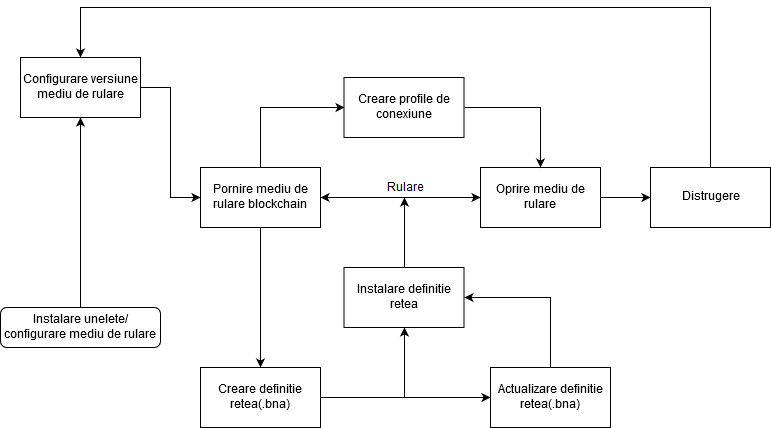
\includegraphics[scale=0.55]{img/deploy.png}
			\caption{Ciclul de via't'a al unei re'tele blockchain}
  			\label{fig:par}
  		\end{center}
  		\end{figure}
  		
  	Re'teaua blockchain ruleaz'a 'intr-un mediu virtual creat cu
ajutorul platformei Docker. Configura'tia ini'tial'a a sistemului din mediul de dezvoltare con'tine 4 imagini Docker: \emph{validating peer}, \emph{ordering} peer, \emph{certificate authority}, \emph{CouchDB}. Mediul virtual con'tine un peer responsabil de validarea 'si salvarea modific'arilor. Comunicarea 'intre peer-uri este asigurat'a de \emph{ordering} peer. 'In final, responsabilitatea pentru emiterea certificatelor de identitate 'si validarea acestora revine \emph{certificate authority}. 'Inregisr'arile din sistem sunt p'astrate 'intr-o baza de date NoSQL care utilizeaz'a imaginea Docker pentru CouchDB\footnote{http://couchdb.apache.org/}. Tabelul \ref{table:img} con'tine imaginile instan'tiate 'in mediul de dezvoltare. Adi'tional acestor imagini, 'in momentul instal'arii defini'tiei re'telei este creat un peer responsabil de rularea codului pentru smart contracts.

\begin{table}[]
\centering
\label{table:img}
\caption{Imagini Docker utilizate 'in mediul de dezvoltare}
\begin{tabular}{|p{7.5cm}|p{6cm}|}
\hline
\hline
Nume imagine                          & Descriere                                               \\ \hline
hyperledger/fabric-peer:x86\_64-1.1.0 & Peer responsabil de validarea 'si salvarea tranzac'tiilor \\ \hline
hyperledger/fabric-ca:x86\_64-1.1.0 & Certificate authority - responsabil'a de emiterea certificatelor de identitate 'in re'tea \\ \hline   
hyperledger/fabric-couchdb:x86\_64-0.4.6 & Baz'a de date pentru 'inregistr'arile din re'tea\\ \hline
hyperledger/fabric-orderer:x86\_64-1.1.0 & Asigur'a comunicarea 'si stabilirea consensului 'intre peer-uri\\ \hline
\end{tabular}
\end{table}

\section{Interac'tiunea cu re'teaua blockchain}
    Dupa instan'tierea re'telei blockchain 'si instalarea defini'tiei re'telei este important'a furnizarea unei metode de interac'tiune cu re'teaua. Utilizarea unui API REST poate permite organiza'tiilor implicate s'a integreze sisteme existente 'in re'teaua blockchain. 
    
    'In acest sens Hyperledger Composer furnizeaz'a o unealt'a pentru instan'tierea unui server REST. Acest server con'tine punctele de acces necesare pentru apelul metodelor CRUD, al tranzactiilor 'si al interog'arilor asupra resurselor. Pe l\^ang'a acestea sunt disponibile metode de sistem pentru citirea istoricului tranzac'tiilor 'si managementul identit'atii participan'tilor. 
    
    Tabelul \ref{table:endpoints} prezint'a punctele de acces la resursele definite 'in sistem. Este posibil'a efectuarea opera'tiilor CRUD asupra asset-urilor 'si participan'tilor din defini'tia re'telei. Opera'tiile efectuate sunt 'inregistrate 'in istoric 'si pot fi observate de participan'tii din re'tea. Invocarea unei tranzac'tii este realizata prin utilizarea metodei POST expus'a de serviciul REST. Tranzac'tiile executate sunt salvate 'intr-un registru al tranzac'tiilor 'si pot fi accesate prin intermediul metodei GET.
    
    
    \begin{table}[H]
    \caption{Puncte de acces 'in re'teaua blockchain}
    \label{table:endpoints}
\centering
\begin{tabular}{|l|l|l|p{2.5cm}|}

\hline
Tip         & Resurs'a                   & Punct de acces             & Metode                       \\ \hline
Asset       & CustomForm                & /CustomForm                & GET, POST, HEAD, PUT, DELETE \\ \cline{2-4} 
            & FormValue                 & /FormValue                 & GET, POST, HEAD, PUT, DELETE \\ \cline{2-4} 
            & MedicalHistory            & /MedicalHistory            & GET, POST, HEAD, PUT, DELETE \\ \cline{2-4} 
            & Patient                   & /Patient                   & GET, POST, HEAD, PUT, DELETE \\ \cline{2-4} 
            & Trial                     & /Trial                     & GET, POST, HEAD, PUT, DELETE \\ \hline
Participant & Agent                     & /Agent                     & GET, POST, HEAD, PUT, DELETE \\ \cline{2-4} 
            & Researcher                & /Researcher                & GET, POST, HEAD, PUT, DELETE \\ \cline{2-4} 
            & ResearcherSite            & /ResearcherSite            & GET, POST, HEAD, PUT, DELETE \\ \cline{2-4} 
            & Supplier                  & /Agent                     & GET, POST, HEAD, PUT, DELETE \\ \cline{2-4} 
            & SupplyOrganisation        & /SupplyOrganisation        & GET, POST, HEAD, PUT, DELETE \\ \hline
Tranzactii  & AddFormData               & /AddFormData               & GET, POST                    \\ \cline{2-4} 
            & AddResearcherToTrial      & /AddResearcherToTrial      & GET, POST                    \\ \cline{2-4} 
            & EnrolPatientTransaction   & /EnrolPatientTransaction   & GET, POST                    \\ \cline{2-4} 
            & RegisterTrialTransaction  & /RegisterTrialTransaction  & GET, POST                    \\ \cline{2-4} 
            & RemoveResearcherFromTrial & /RemoveResearcherFromTrial & GET, POST                    \\ \hline
\end{tabular}
\end{table}

Adi'tional acestor puncte de acces sunt create puncte de acces pentru executarea interog'arilor definite 'in re'tea. Aceste puncte de acces expun metode GET pentru executarea 'si preluarea rezultatului interog'arilor. Punctele de acces expuse de serverul REST sunt definite 'in tabelul \ref{table:query}

\begin{table}[H]
\centering
\label{table:query}
\caption{Puncte de acces interog'ari}
\begin{tabular}{|l|l|}
\hline
\hline
Interog'ari                        & Punct de acces                             \\ \hline
selectDataForCustomForm           & /queries/selectDataForCustomForm           \\ \hline
selectDataForCustomFormAndPatient & /queries/selectDataForCustomFormAndPatient \\ \hline
selectFilesByTrial                & /queries/selectFilesByTrial                \\ \hline
selectPatientsForTrial            & /queries/selectPatientsForTrial            \\ \hline
selectCustomFormsByTrial          & /queries/selectCustomFormsByTrial          \\ \hline
selectTrialsByResponsible & /queries/selectTrialsByResponsible \\ \hline
selectHistoryByUser & queries/selectHistoryByUser\\ \hline
selectHistoryByResource & queries/selectHistoryByResource\\ \hline
\end{tabular}
\end{table}
    
\section{Management utilizatori}
    Identitatea utilizatorilor este gestionat'a la nivelul serverului REST care ruleaza 'in modul cu utilizatori multiplii. Configurarea unui server rest 'in modul cu utilizatori multiplii este prezentat'a 'in sec'tiunea \ref{multi:rest}.  Dup'a activarea modului cu utilizatori multiplii orice 'incercare de apel a metodelor expuse de serverul REST f'ar'a ca utilizatorul s'a fie autentificat are ca rezultat r'aspunsul din figura \ref{fig:401}.
  	
  	    \begin{figure}[H]
		\begin{center}
			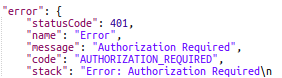
\includegraphics[scale=0.9]{img/err401.png}
			\caption{R'aspuns server REST pentru utilizator neautorizat}
  			\label{fig:401}
  		\end{center}
  		\end{figure}
    
    'In acest fel este permis accesul doar utilizatorilor autentifica'ti. Astfel tranzac'tiile efectuate 'in sistem nu sunt semnate folosind identitatea administratorului re'telei. 'In schimb fiec'arui utilizator 'ii este asociat un \emph{wallet} 'in care sunt stocate identit'a'tile asociate utilizatorului autentificat. Fiecare utilizator semneaz'a astfel tranzac'tiile folosind identitatea setat'a ca default 'in \emph{wallet}-ul de'tinut de el. Utiliz\^and aceasta abordare pot fi aplicate reguli de acces asupra participan'tilor, asigur\^andu-se astfel protejarea datelor cu caracter sensibil. 
    
    Procesul de autentificare al unui utilizator implica 5 componente din arhitectura sistemului. Interac'tiunea dintre componente este prezentat'a cu ajutorul unei diagrame de secven't'a ilustrat'a 'in figura \ref{fig:auth-seq}. Procesul reprezentat 'in figur'a este realizat 'in cazul 'in care utilizatorul are deja definit'a o identitate 'in \emph{wallet}-ul s'au 'si aceasta poate fi citit'a de serverul REST. Dup'a terminarea procesului de autentificare token-ul generat de serviciul extern este stocat cu ajutorul unui \emph{cookie} 'in browser-ul utilizatorului. Acest token specific'a server-ului REST identitatea utilizatorului. 

 \begin{figure}[H]
		\begin{center}
			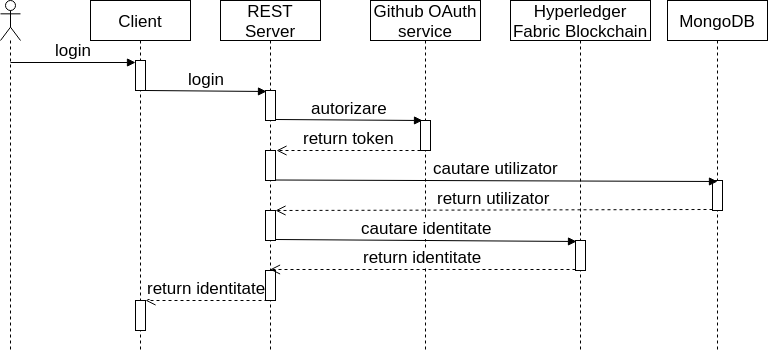
\includegraphics[scale=0.5]{img/auth-seq.png}
			\caption{Procesul de  autentificare al unui utilizator}
  			\label{fig:auth-seq}
  		\end{center}
  		\end{figure}
  	
    Creden'tialele utilizatorului sunt gestionate de serviciul exetern de autentificare. Acesta furnizeaz'a un token prin care serverul REST diferen'tiaza utilizatorii din sistem. Asocierile dintre utilizatori 'si token-urile de acces sunt p'astrate 'in memoria intern'a a serverului REST. Din acest motiv 'in momentul 'in care instan'ta serverului este oprit'a, asocierile dintre identit'a'tile utilizatorilor 'si token-ul de autentificare sunt pierdute. Acesta problem'a este rezolvat'a 'insa prin utilizarea unei baze de date MongoDB al'aturi de instan'ta server-ului pentru a re'tine token-urile utilizatorilor din sistem. Astfel, aceste asocieri sunt p'astrate permanent, chiar 'si dupa un restart al serverului.
    
    Procesul de asociere a unei identit'a'ti 'in re'teaua blockchain presupune parcurgerea urm'atorilor pa'si:
    \begin{itemize}
        \item Crearea unui participant 'in re'teaua blockchain
        \item Emiterea unei identit'a'ti pentru participant
        \item Crearea unui card de acces 'in re'tea folosind identitatea emisa
        \item Importarea cadrului 'in \emph{wallet}-ul unui utilizator autentificat
    \end{itemize}
    
    Din punctul de vedere al utilizatorului procesul de asociere al contului s'au din cadrul aplica'tiei externe la re'teaua blockchain trebuie s'a fie c\^at mai automatizat 'si sigur. De aceea, responsabilitatea de creare a participan'tilor 'in re'teaua blockchain revine administratorului re'telei. Utilizatorii sistemului primesc un cod de inrolare cu ajutorul c'aruia pot asocia o anumit'a identitate contului folosit 'in aplicatie extern'a de autentificare. Astfel, din punctul de vedere al utilizatorului pa'sii descri'si mai sus se rezum'a doar la introducerea codului furnizat de organiza'tia din care face parte, folosind pagina prezentat'a 'in figura \ref{fig:app-bind}.
    
     \begin{figure}[H]
		\begin{center}
			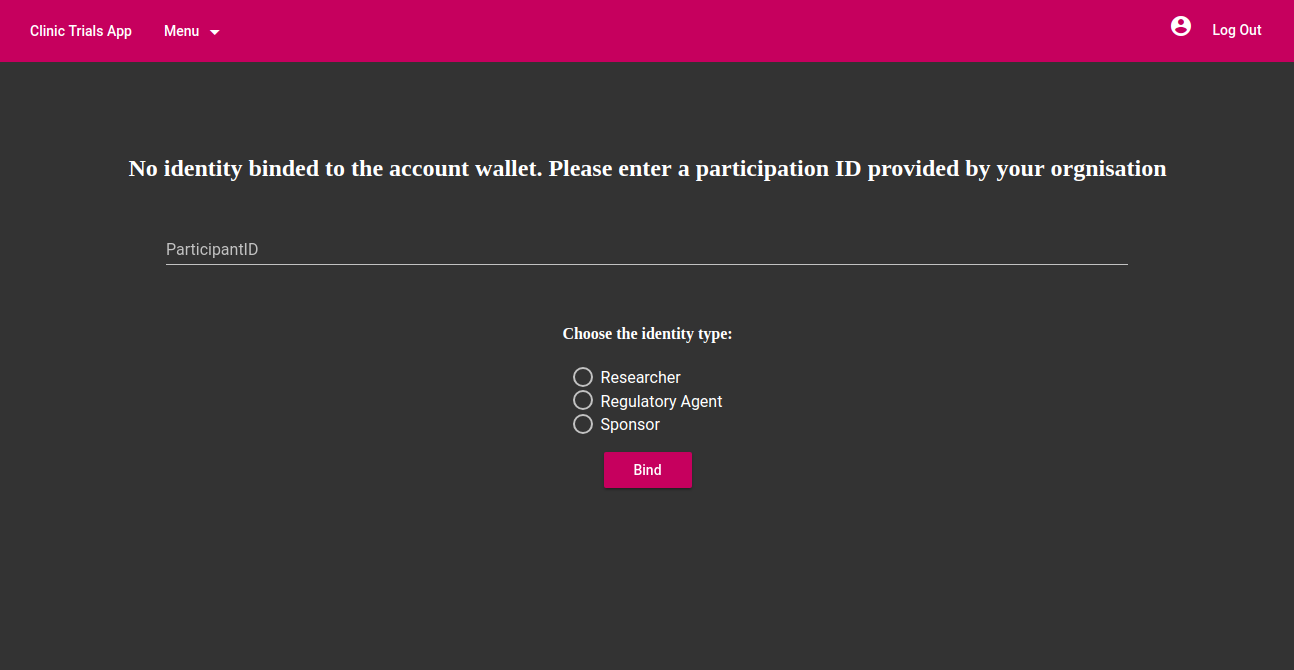
\includegraphics[scale=0.3]{img/bind.png}
			\caption{Pagina pentru asocierea identit'a'tii unui utilizator utilizator}
  			\label{fig:app-bind}
  		\end{center}
  		\end{figure}
  	
  	Procesul de asociere al identit'a'tii la contul din aplica'tia extern'a de autentificare este prezentat 'in diagrama de secven't'a din figura \ref{fig:assoc}. Codul de 'inrolare primit de utilizator reprezint'a ID-ul unui participant creat 'in re'teaua blockchain.
  	
  	 \begin{figure}[H]
		\begin{center}
			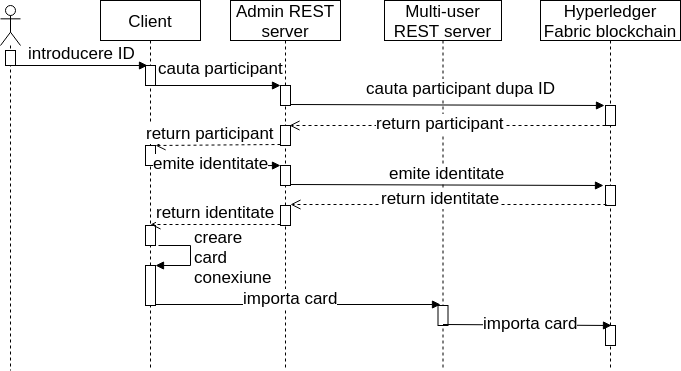
\includegraphics[scale=0.55]{img/seq-usr-cr.png}
			\caption{Procesul de asociere al unei identit'a'ti}
  			\label{fig:assoc}
  		\end{center}
  		\end{figure}
  	
  	Dup'a ce utilizatorul introduce ID-ul furnizat aplica'tia client verific'a existen'ta acestuia printr-un apel la serverul REST. Acest apel interoghez'a registrul de participan'ti stocat 'in re'teaua blockchain 'si returneaz'a detaliile despre participant dac'a acesta exist'a. Aplica'tia client utilizeaz'a informa'tiile despre participant pentru a efectua un apel de emitere a identit'a'tii pentru un participant. Re'teaua blockchain genereaza cheile private 'si publice ale participantului 'si returneaza aplica'tiei client informa'tiile necesare pentru a genera un card de conexiune. Acest card de conexiune este importat 'in final 'in \emph{wallet}-ul unui utilizator. 'In urma efectu'arii acestor opera'tii utilizatorul poate folosi identitatea asociata contului s'au pentru a semna tranzac'tiile din sistem.	
  	
  	\section{Arhitectura aplica'tiei client}
  	
  	Aplica'tia client a sistemului este implementata cu ajutorul framework-ului Angular. 'In continuare sunt prezentate aspecte legate de modul de implementare al serviciilor responsabile de comunicarea cu serverul REST 'si componentele principale ale aplica'tiei client.
  	
  	\subsection{Servicii HTTP}
  	
  	Comunicarea interfe'tei web cu re'teaua blockchain se realizeaz'a prin intermediul server-ului REST. Cu ajutorul modulului \emph{HttpClient} sunt implementate apelurile de metode REST din aplica'tia client. 
  	
  	 	
  	  	 \begin{figure}[H]
		\begin{center}
			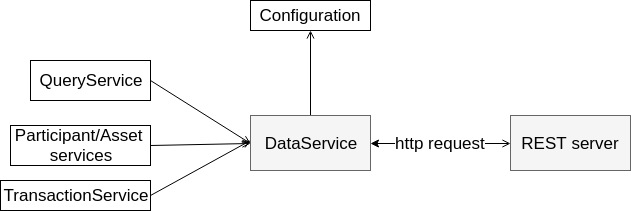
\includegraphics[scale=0.55]{img/data-rest.png}
			\caption{Serviciul HTTP al aplica'tiei client}
  			\label{fig:data}
  		\end{center}
  		\end{figure}
  		
  	Figura \ref{fig:data} prezint'a elementele principale ale aplica'tiei client, responsabile de interac'tiunea cu serverul rest. Apelurile REST sunt efectuate prin intermediul serviciului generic DataService. Acest serviciu este injectat mai departe 'in serviciile rescponsabile de apeluri de interog'ari, opera'tii CRUD pe resurse sau apeluri de tranzac'tii. Componenta \emph{Configuration} con'tine constante pentru identificarea server-ului REST, simplific\^and opera'tia de modificare a adresei spre server. 'In figura \ref{config} se pot observa constantele definite pentru configurarea accesului la serverul REST 'si modul simplu de modificare al acestora.
  	\begin{figure}[H]
  	\begin{lstlisting}[style=htmlcssjs]
@Injectable()
export class Configuration {
    public ApiIP: string = "http://localhost";
    public ApiPort: string = "3000";
    public AdminApiPort: string = "3001";
    public Server: string = this.ApiIP+":"+this.ApiPort;
    public AdminServer: string = this.ApiIP+":"+this.AdminApiPort;
    public ApiUrl: string = "/api/";
    public ServerWithApiUrl = this.Server + this.ApiUrl;
    public AdminServerWithApiUrl = this.AdminServer + this.ApiUrl; 
}

  	\end{lstlisting}
  	\caption{Component'a de configurare}
  	\label{config}
  	\end{figure}


\subsection{Componentele aplica'tiei client}
    Paginile aplica'tiei client sunt alc'atuite din componente g\^andite pentru a beneficia de pe urma posibilit'a'tilor de refolosire a acestora. Figura \ref{fig:ui-arh} ilustreaz'a componentele aplica'tiei client 'si dependin'tele dintre acestea. 
    \begin{figure}[H]
		\begin{center}
			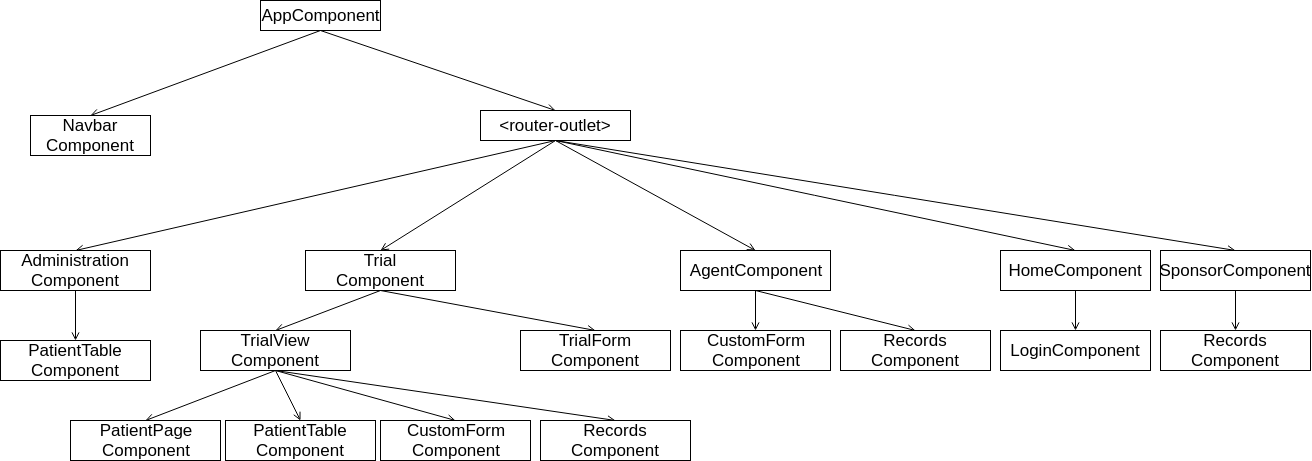
\includegraphics[scale=0.32]{img/ui-arh.png}
			\caption{Diagrama de componente a aplica'tiei client}
  			\label{fig:ui-arh}
  		\end{center}
  	\end{figure}

Componenta r'ad'acina a aplica'tiei de'tine responsabilitatea de randare a \emph{router-outlet}. Componenta router-outlet face parte din mecanismul Angular de rutare al aplica'tiei client. 'In func'tie de ruta de naviga'tie router-outlet afi'seaz'a o anumit'a component'a a aplica'tiei. 

Posibilitatea de refolosire a codului este asigurat'a prin implementarea de directive Angular 'si componente. Componentele reprezint'a o extensie a directivelor. Un exemplu 'in acest sens este implementarea unui tabel pentru pacien'ti sub forma unei componente. Defini'tia unei astfel de componente 'incepe folosind decoratorul \emph{@Component} exemplificat 'in figura \ref{at-comp}. Proprietatea \emph{selector} specific'a numele tag-ului HTML care poate fi folosit pentru a instan'tia componenta.

  	\begin{figure}[H]
  	\begin{lstlisting}[style=htmlcssjs]
@Component({
    selector: 'patient-table',
    templateUrl: 'patient-table.component.html'
})
export class PatientTableComponent implements OnInit {
    @Input() allPatientsDataSource: MatTableDataSource<Patient>;
    @Input() adminMode: boolean;
    @Input() idTrial: string;
...
  	\end{lstlisting}
  	\caption{Decoratorul @Component}
  	\label{at-comp}
  	\end{figure}
  	
Parametrii care au aplicat decoratorul \emph{@Input()} pot fi referi'ti ca atribute 'in interiorul tag-urilor HTML pentru a transmite valori componentei. Astfel, componenta prezentat'a mai sus poate fi folosit'a 'in interiorul unei alte componente prin utilizarea sintaxei prezentate 'in figura \ref{reuse}.
  	\begin{figure}[H]
  	\begin{lstlisting}[style=htmlcssjs]
 <patient-table [allPatientsDataSource]="allPatientsDataSource"
 [adminMode]=false [idTrial]="trial.idTrial"></patient-table>
  	\end{lstlisting}
  	\caption{Reutilizarea unei componente Angular}
  	\label{reuse}
  	\end{figure}
  	


\newpage
\thispagestyle{empty}
\mbox{}

\chapter{Testare 'si Validare}

    Calitatea produsului sau serviciului oferit poate fi analizat'a prin testarea obiectiv'a a func'tionalit'a'tilor furnizate de produs. 'In continuare sunt prezentate metodele de testare folosite pentru verificarea calit'a'tii sistemului.
    
    \section{Testarea re'telei blockchain}
    Are ca scop testarea defini'tiei re'telei blokchain 'si a performan'tei acesteia. Pentru testarea defini'tiei unei re'tele 'si pentru validarea functionalit'a'tilor acesteia inainte de instalarea aplica'tiei 'in productie, dezvoltatorii au la dispozitie tool-ul \textbf{Composer Playground} disponibil pentru utilizare fie online\footnote{http://composer-playground.mybluemix.net/}, fie 'intr-un mediu de dezvoltare local.
    
         \begin{figure}[H]
		\begin{center}
			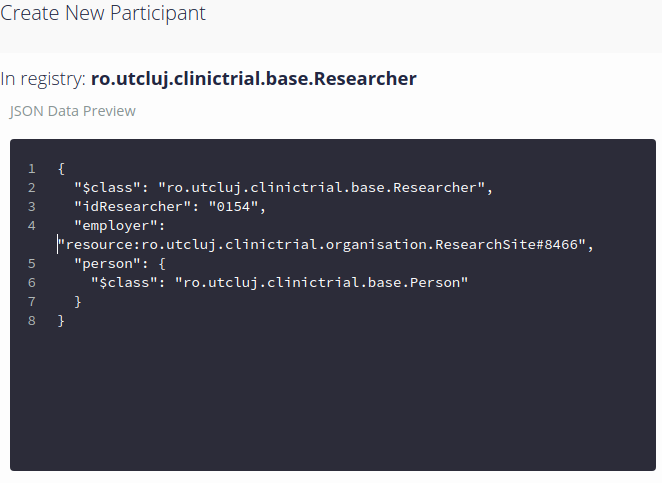
\includegraphics[scale=0.35]{img/play-add.png}
			\caption{Testare func'tionalitate de ad'augare a unui nou participant}
  			\label{fig:play-add}
  		\end{center}
  		\end{figure}
    Acest tool ofer'a posibilitatea dezvoltatorilor de a testa 'in cadrul platformei defini'tia re'telei. Cu ajutorul platformei pot fi testate opera'tii CRUD, fiind puse la dispozi'tie exemple 'si posibilitatea de a adauga date aleatoare pentru testare similar cu cele prezentate 'in figura \ref{fig:play-add}.

    O func'tionalitate important'a oferit'a de Composer Playground este posibilitatea de a testa logica tranzac'tiilor. Figura \ref{fig:play-tranz} prezint'a functionalitatea oferit'a de platforma pentru testarea logicii tranzac'tiilor. Sunt oferite, de asemenea, exemple ale parametrilor necesari pentu apelul tranzac'tiilor. Platforma ofer'a posibilitatea de interogare a istoricului tranzac'tiilor pentru validarea mecanismului de memorare al istoricului tranzactiilor.
    
    
         \begin{figure}[H]
		\begin{center}
			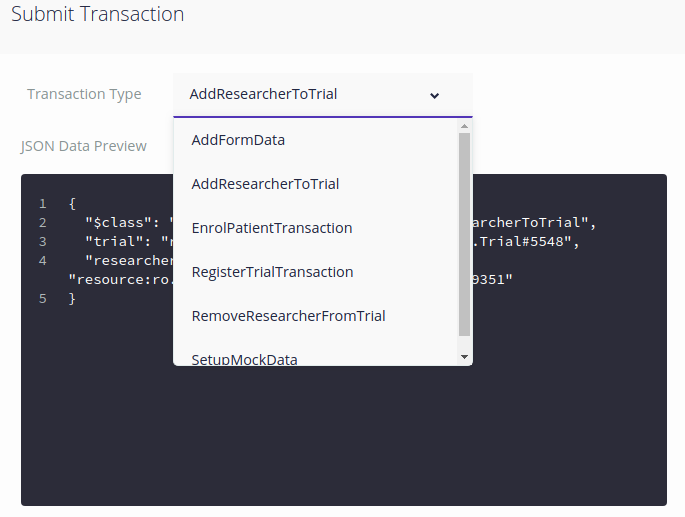
\includegraphics[scale=0.5]{img/play-tranz.png}
			\caption{Testare apeluri tranzac'tii}
  			\label{fig:play-tranz}
  		\end{center}
  		\end{figure}
  		
    \section{Testare la nivelul API-ului REST} Comunicarea 'intre interfa'ta utilizator 'si re'teaua blockchain se realizeaz'a prin intermediul unui server REST. Server-ul REST creat cu ajutorul Hyperledger Composer ofer'a posibilitatea de testare a metodelor din API prin intermediul unei documenta'tii web create cu ajutorul uneltei \textbf{Swagger}\footnote{https://swagger.io/}. Figura \ref{fig:swagger} ilustreaza un model de documenta'tie generat pentru API-ul sistemului de management al studiilor clinice. Documenta'tia generat'a prezint'a metodele expuse de serverul REST, exemple de apeluri 'si ofer'a 'in acela'si timp posibilitatea de a apela metodele generate. Aceste aspecte simplific'a procesul de documentare al unui API. Dezvoltatorii interfe'tei utilizator pot prelua documenta'tia generata 'si o pot utiliza pentru a integra inter'fata utilizator cu re'teaua blockchain.
    
             \begin{figure}[H]
		\begin{center}
			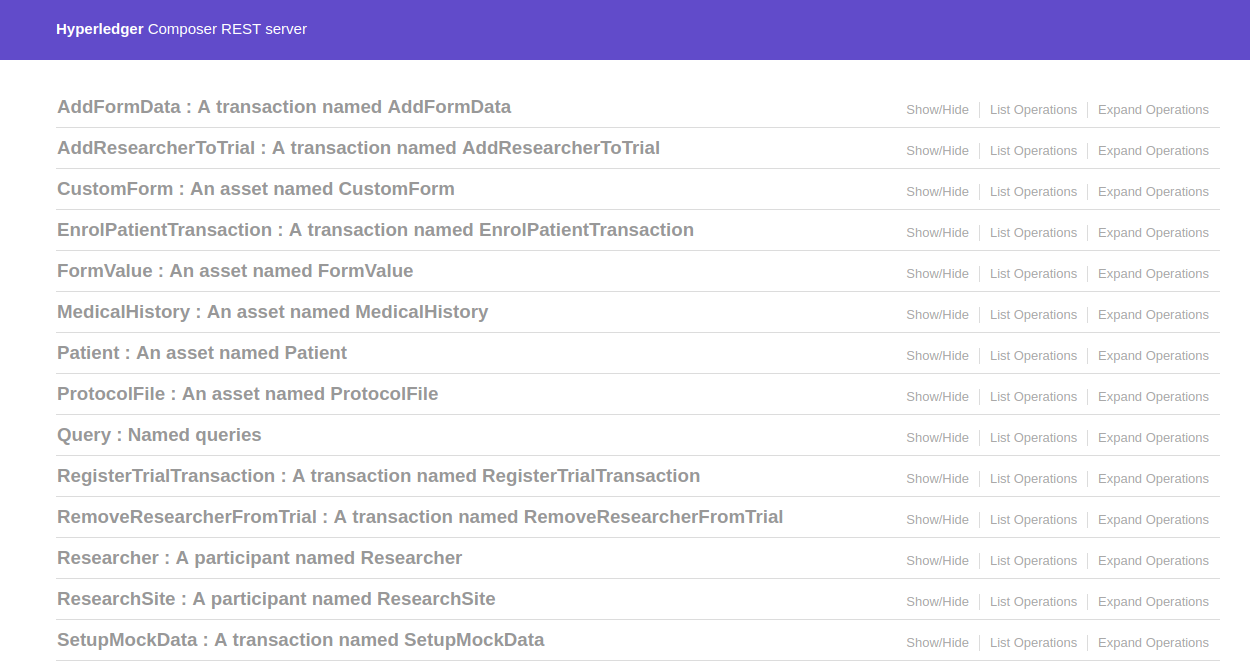
\includegraphics[scale=0.35]{img/swagger.png}
			\caption{Documenta'tie API generat'a folosind Swagger}
  			\label{fig:swagger}
  		\end{center}
  		\end{figure}
  		
  	\section{Testare la nivelul aplica'tiei client}
  	La nivelul aplica'tiei client, framework-ul Angular pune la dispozi'tie unealta pentru testare \textbf{Karma}\footnote{http://karma-runner.github.io/2.0/index.html} al'aturi de framework-ul Jasmine\footnote{https://jasmine.github.io/}. Aceasta unealt'a permite scrierea de scenarii de testare a componentelor interfe'tei utilizator, a metodelor definite 'si a serviciilor din aplica'tia client. Anexa \ref{app:test} prezint'a un exemplu cod scris 'in limbajul JavaScript pentru testarea unei componente din interfa'ta utilizator. Pentru executarea testelor definite 'in aplica'tia client se utilizeaz'a comanda:
  \definecolor{light-gray}{gray}{0.80}
  	\begin{lstlisting}[backgroundcolor=\color{light-gray}]
    ng test
    \end{lstlisting}
    Aceasta comand'a scaneaz'a directorul surs'a al aplica'tiei pentru a g'asi fi'sierele 'in care sunt definite cazurile de testare. Aceste fi'siere folosesc extensia ".spec.ts". Rezultatele testelor pot fi vizualizate pe interfa'ta web a mecanismului de testare. Figura \ref{fig:karma} prezint'a rezultatul ob'tinut 'in urma efectuarii unui test simplu de instan'tiere a unei componente.
    
                 \begin{figure}[H]
		\begin{center}
			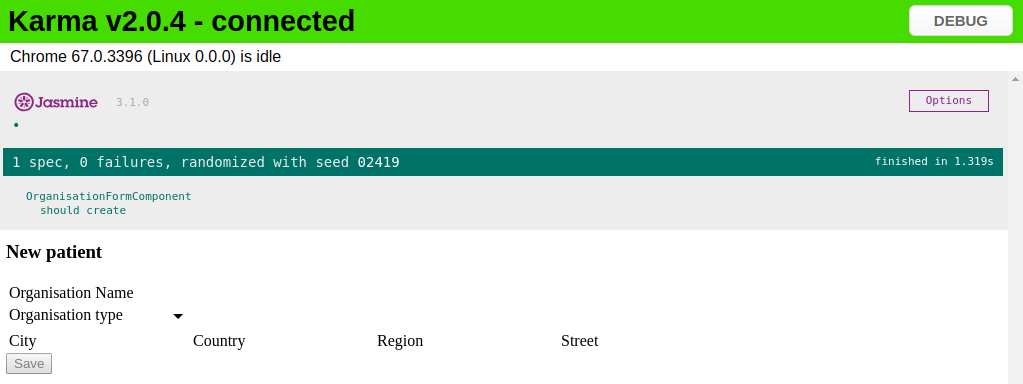
\includegraphics[scale=0.35]{img/karma.png}
			\caption{Interfa'ta web pentru rulare teste}
  			\label{fig:karma}
  		\end{center}
  		\end{figure}
  		
    
    
      	
\chapter{Manual de Instalare 'si Utilizare}
\section{Cerinte preliminare}
Instalarea uneltelor de dezvoltare a re'telei blockchain 'si a interfe'tei utilizator necesit'a indeplinirea urm'atoarelor cerin'te preliminare :
\begin{itemize}
    \item \textbf{Sistem de operare}: Ubuntu Linux 14.04 / 16.04 LTS (both 64-bit), Mac OS 10.12
    \item \textbf{Docker}: Version 17.03+
    \item \textbf{Docker-Compose}: Version 1.8+
    \item \textbf{Node}: 8.9+
    \item \textbf{npm}: 5.x+
    \item \textbf{git}: 2.9.x+ 
    \item \textbf{Python}: 2.7.x+
    \item \textbf{Angular CLI}: 6.x.x+
    \item \textbf{MongoDB}: 4.0+
\end{itemize}

\section{Instalare}
\definecolor{light-gray}{gray}{0.80}
\subsection{Instalare mediu de rulare Hyperledger Fabric}
    'In continuare sunt prezenta'ti pa'sii necesari pentru instalarea resurselor mediului de rulare 'si pa'sii necesari pentru pornirea acestuia. 
    \begin{enumerate}
        \item 'Intr-un director la alegere('in acest caz \textbf{/fabric-dev-servers}) sunt desc'arcate resursele Hyperledger Fabric folosind comenzile:
    \begin{lstlisting}[backgroundcolor=\color{light-gray}]
mkdir ~/fabric-dev-servers && cd ~/fabric-dev-servers

curl -O https://raw.githubusercontent.com/hyperledger/compose
r-tools/master/packages/fabric-dev-servers/fabric-dev-servers
.tar.gz tar -xvf fabric-dev-servers.tar.gz
    \end{lstlisting}
    
    \item Este executat script-ul furnizat pentru desc'arcarea imaginilor Docker execut\^and urmatoarele comenzi:
    \begin{lstlisting}[backgroundcolor=\color{light-gray}]
cd ~/fabric-dev-servers
./downloadFabric.sh
    \end{lstlisting}
    \item Dup'a executarea comenzilor sunt instalate toate resursele necesare pornirii mediului de rulare Hyperledger Fabric. Pentru pornirea mediului de rulare este necesar'a pornirea imaginilor Docker desc'arcate anterior. Acest lucru este realizat prin executarea urmatoarelor script-uri furnizate:
    \begin{lstlisting}[backgroundcolor=\color{light-gray}]
./startFabric.sh
./createPeerAdminCard.sh
    \end{lstlisting}
    \end{enumerate}

\subsection{Instalare Hyperledger Composer}
    Uneltele furnizate de Hyperledger composer sunt instalate cu ajutorul uneltei \textbf{npm}. Este necesara instalarea global'a a urmatoarelor pachete:
    \begin{itemize}
        \item \textbf{Composer CLI}:
            \begin{lstlisting}[backgroundcolor=\color{light-gray}]
npm install -g composer-cli
            \end{lstlisting}
        \item \textbf{Composer REST server}:
            \begin{lstlisting}[backgroundcolor=\color{light-gray}]
npm install -g composer-rest-server
            \end{lstlisting}
    \end{itemize}
    
\subsection{Instalare defini'tie re'tea}

Defini'tia re'telei blockchain este furnizat'a sub forma unui fi'sier cu extensia .bna. Instalarea defini'tiei 'intr-un peer din re'tea presupune urm'atorii pa'si:
    \begin{enumerate}
        \item Este importat fi'sierul PeerAdmin@fabric-network.card ob'tinut urm\^and pa'sii de instalare a mediului de rulare Hyperledger Fabric. Pentru a importa acest fi'sier se foloseste urmatoarea comanda:
        \begin{lstlisting}[backgroundcolor=\color{light-gray}]
composer card import -f PeerAdmin@fabric-network.card
            \end{lstlisting}
        \item Se instaleaz'a fi'sierul cu defini'tia re'telei folosind urmatoarea comand'a:
        \begin{lstlisting}[backgroundcolor=\color{light-gray}]
composer network install -c PeerAdmin@fabric-network -a 
clinic-trial-network1.0.0.bna
        \end{lstlisting}
        \item Pentru a porni defini'tia re'telei instalate se execut'a urm'atoarea comanda:
         \begin{lstlisting}[backgroundcolor=\color{light-gray}]
composer network start --networkName clinic-trial-network 
--networkVersion 1.0.0 -A admin -S adminpw -c 
PeerAdmin@fabric-network
        \end{lstlisting}
        \item Pasul anterior creaz'a un card de conexiune la peer-ul din re'teaua blockchain sub numele \textbf{admin@clinic-trial-network.card}. Pentru a putea interac'tiona cu defini'tia re'telei este necesar'a importarea acestui card folosind comand'a:
         \begin{lstlisting}[backgroundcolor=\color{light-gray}]
composer card import -f admin@clinic-trial-network.card
        \end{lstlisting}
    \end{enumerate}

\subsection{Configurare server REST}
Sistemul utilizeaz'a dou'a servere REST pentru a permite utilizatorilor s'a interac'tioneze cu re'teaua blockchain utiliz\^and inter'fata utilizator. Unul din servere ruleaz'a 'in modul administrator av\^and rolul de a crea identit'a'ti 'in re'teaua blockchain. Cel'alalt server ruleaz'a 'in modul cu utilizatori multiplii.
\subsubsection{Configurare server REST 'in modul administrator}
Pentru instan'tierea unui server REST 'in modul administrator este utilizat'a urm'atoarea comand'a:
  \begin{lstlisting}[backgroundcolor=\color{light-gray}]
composer-rest-server -c admin@clinic-trial-network -n never -p 3001
        \end{lstlisting}

\subsubsection{Configurare server REST 'in modul cu utilizatori multiplii}\label{multi:rest}

Pentru pornirea unui server REST 'in modul cu utilizatori multiplii sunt necesari urm'atorii pa'si, al'aturi de urmatoarele configur'ari:
\begin{enumerate}
    \item Serviciul de stocare permanent'a a utilizatorilor este pornit folosind comenzile:
      \begin{lstlisting}[backgroundcolor=\color{light-gray}]
sudo service mongod start
mongo
       \end{lstlisting}
    \item Pentru pornirea serverului REST 'in modul cu utilizatori multiplii se execut'a scriptul furnizat. Con'tinutul scriptului este disponibil 'in anexa \ref{multiusr}.
     \begin{lstlisting}[backgroundcolor=\color{light-gray}]
./start-multi-rest-server
       \end{lstlisting}
       
\end{enumerate}

\subsection{Configurare interfa't'a utilizator}
'Inainte de pornirea serverului pentru interfa'ta utilizator este necesar'a instalarea dependin'telor acesteia folosind comanda:
\begin{lstlisting}[backgroundcolor=\color{light-gray}]
npm install
       \end{lstlisting}
       
Instan'tierea serverului pentru interfa'ta utilizator este realizat'a prin utilizarea\\ comenzii:       
\begin{lstlisting}[backgroundcolor=\color{light-gray}]
ng serve
\end{lstlisting}

\section{Manual de utilizare}
'In aceast'a sec'tiune se prezint'a pe scurt unele detalii legate de utilizarea aplica'tiei. Aplica'tia a fost g\^andit'a 'in a'sa fel 'inc\^at s'a fie simplu de utilizat, dar unele clarificari referitoare la func'tionalit'a'ti sunt necesare.
Autentificarea utilizatorului se efectueaza prin utilizarea butonului de Login aflat pe pagina de pornire. Utilizatorul este redirec'tionat spre serviciul de autentificare extern dup'a ap'asarea butonului.
         \begin{figure}[H]
		\begin{center}
			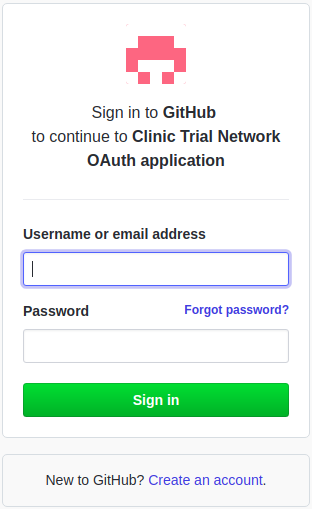
\includegraphics[scale=0.5]{auth.png}
			\caption{Pagina de autentificare a serviciului extern}
  			\label{fig:auht-ext}
  		\end{center}
  		\end{figure}

Dup'a autentificare utilizatorii sunt redirec'tiona'ti 'in func'tie de rolul lor spre paginile principale. Cercet'atorii sunt redirec'tionati spre pagina care con'tine studiile clinice la care au acces.
         \begin{figure}[H]
		\begin{center}
			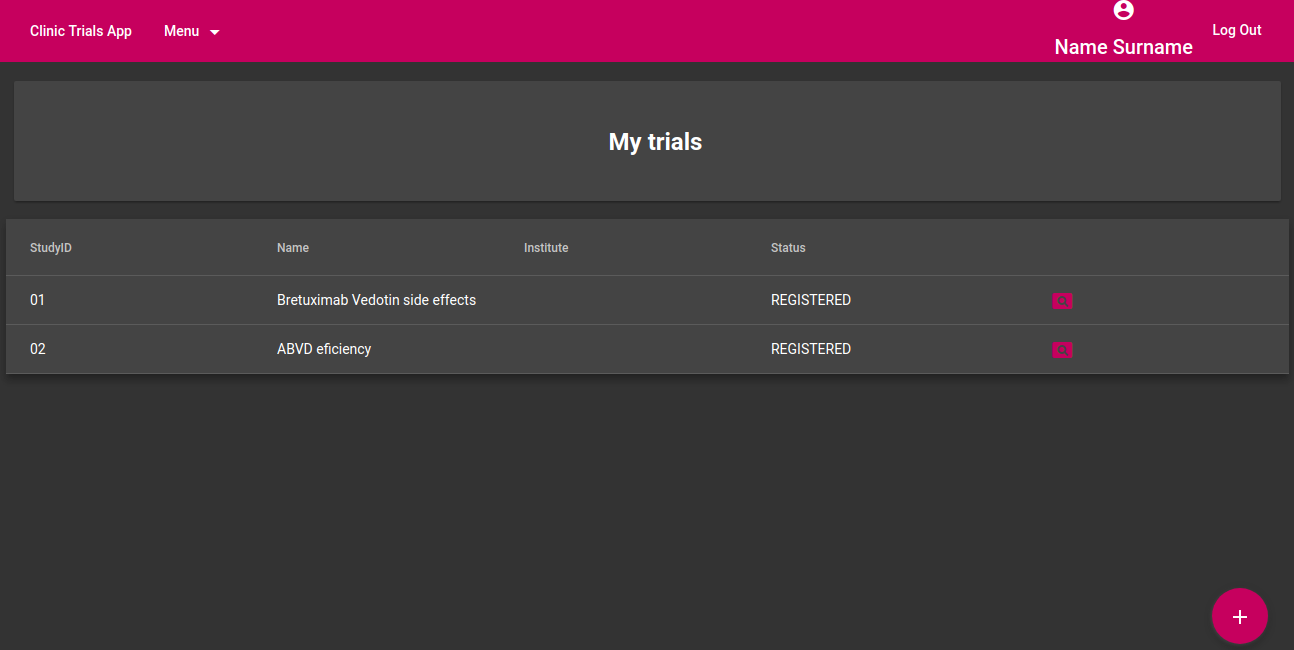
\includegraphics[scale=0.35]{trial.png}
			\caption{Pagina principal'a a cercetatorului}
  			\label{fig:traials}
  		\end{center}
  		\end{figure}

Adaugarea de resurse 'in sistem, fie studii clinice noi, fie pacien'ti sau incarcarea de fi'siere se poate realiza cu ajutorul butonului din partea dreapta-jos a paginii asociate resursei respective. Acest buton este vizibil 'in figura \ref{fig:traials}. 

Diferite opera'tii pot fi realizate asupra resurselor utiliz\^and butoanele asociate fiec'arei 'inregistr'ari din tabelele de date. Aceste butoane sunt marcate 'in figura \ref{fig:acts}. 'In func'tie de resursa 'si drepturile utilizatorului sunt puse la dispozi'tie prin aceste butoane opera'tii de editare, 'stergere sau vizualizare a unei resurse.

         \begin{figure}[H]
		\begin{center}
			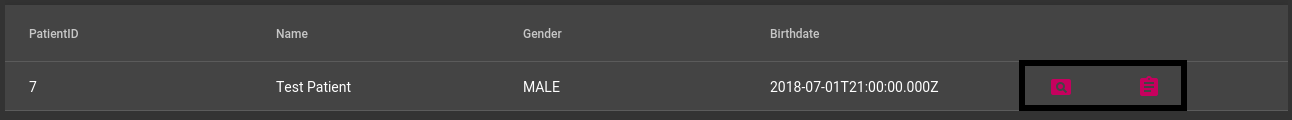
\includegraphics[scale=0.35]{actions.png}
			\caption{Butoane pentru opera'tii asupra inregistr'arilor}
  			\label{fig:acts}
  		\end{center}
  		\end{figure}
  		
Dupa accesarea unui studiu clinic din pagina principal'a a cercet'atorului prezentat'a 'in figura \ref{fig:traials} utilizatorul este redirectionat spre pagina dedicat'a studiului clinic. Aceasta pagina con'tine o serie de \emph{tab}-uri, fiecare oferind func'tionalit'a'ti 'si servicii 'in cadrul unui studiu clinic. 'In figura \ref{fig:overview} se poate observa pagina principal'a din cadrul unui studiu clinic 'si \emph{tab}-urile aociate acestuia.

         \begin{figure}[H]
		\begin{center}
			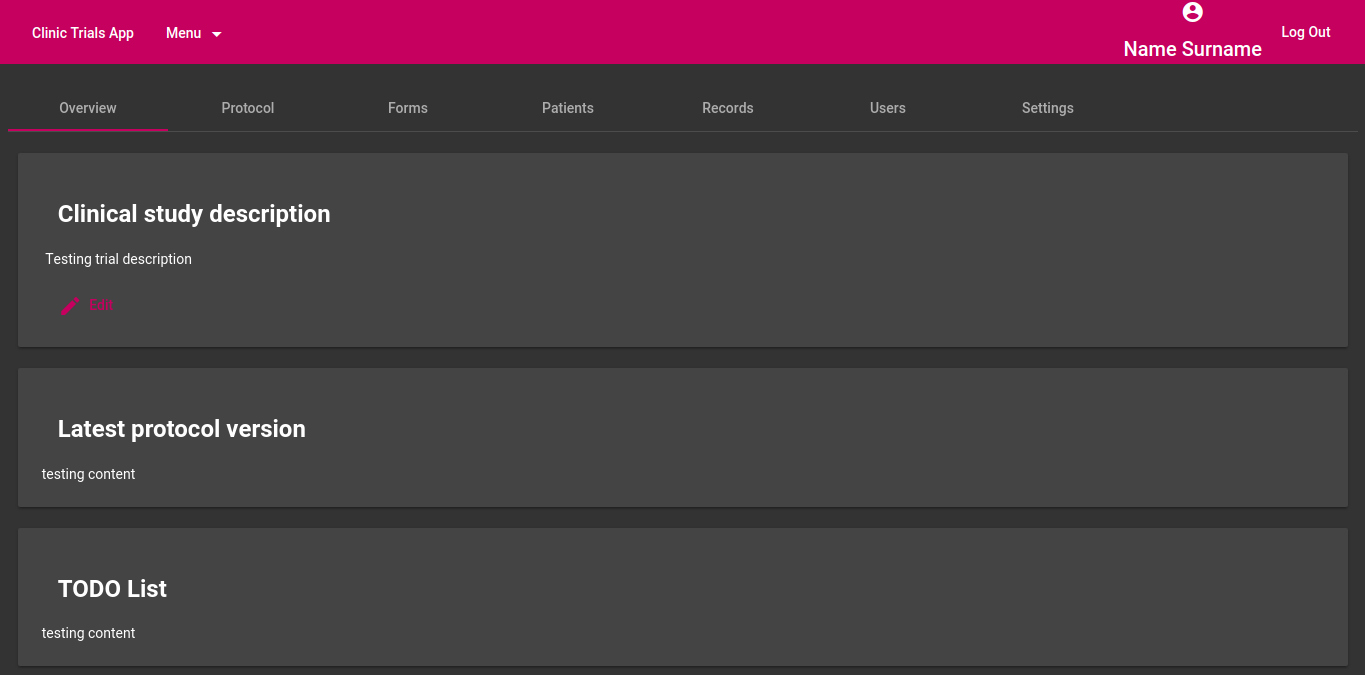
\includegraphics[scale=0.35]{img/trial-overview.png}
			\caption{Pagina dedicat'a studiilor clinice}
  			\label{fig:overview}
  		\end{center}
  		\end{figure}
  Tab-urile puse la dispozi'tia cercet'atorilor care au drepturile de acces necesare la un studiu clinic sunt:
 \begin{itemize}
     \item \textbf{Overview}: Pagina de prezentare a unui studiu clinic. Con'tine informa'tii generale despre un studiu clinic
     \item \textbf{Protocol}: Ofer'a servicii de management a fi'sierelor de protocol
     \item \textbf{Forms}: Crearea de formulare personalizate 'si gestionarea formularelor deja create este posibil'a 'in cadrul acestei pagini.
     \item \textbf{Patients}: Ofer'a servicii pentru managementul pacien'tilor dintr-un studiu clinic.
     \item \textbf{Users}: Permite definirea utilizatorilor care au drepturi de acces la studiul clinic.
     \item \textbf{Settings}: Con'tine set'ari generale aplicate studiului clinic.
 \end{itemize}

\chapter{Concluzii}

Capitolul prezint'a rezultatele ob'tinute 'in urma implement'arii sistemului de management al studiilor clinice. Este prezentat'a o analiz'a a sistemului al'aturi de unele posibile dezvolt'ari ulterioare ale acestuia.

\section{Rezultate ob'tinute}

    Sistemul pentru managementul studiilor clinice simplific'a modul de interac'tiune 'intre organiza'tiile implicate 'in procesul de management 'si reglementare al studiilor clinice. Prin utilizarea unei arhitecturi distribuite 'in care fiecare participant din re'tea de'tine o copie a datelor colectate 'in sistem, nivelul de incredere 'in corectitudinea datelor colectate este 'imbun'at'a'tit. Unele din caracteristicile sistemului implementat sunt:
    \begin{itemize}
        \item \textbf{Protec'tia datelor cu caracter personal:} Listele de acces definite 'in aplica'tie asigur'a faptul ca participan'tii au acces doar la informa'tiile definite 'in regulile de acces aplicate asupra lor
        \item \textbf{Partajarea datelor:} Procesul de partajare a datelor este simplificat 'si realizat prin mijloace sigure. Acest lucru este realizat prin utilizarea unei baze de date distribuite.
        \item \textbf{Managementul utilizatorilor:} Accesul utilizatorilor la resursele sistemului este gestionat la nivelul server-ului. Fiecare utilizator realizeaz'a opera'tii 'in sistem utiliz\^and identitatea de'tinut'a.
        \item \textbf{Stocarea sigura a fi'sierelor:} Fi'sierele stocate 'in cadrul re'telei blockchain sunt imutabile. Modificarea lor nu poate avea loc f'ar'a a fi l'asat'a o urma 'in sistem.
        \item \textbf{Reglementarea studiilor clinice:} Agen'tii de reglementare 'si sponsorii au acces la istoricul opera'tiilor efectuate 'in sistem. Astfel este eficientizat procesul de aplicare a regulilor asupra studiilor clinice.
        \item \textbf{Colectarea datelor:} Sistemul ofer'a flexibilitate 'in ce prive'ste datele colectate de cercet'atori 'in cadrul unui studiu clinic. Cercet'atorii au posibilitatea de a-'si defini propriile formulare de colectare a datelor.
    \end{itemize}
    
    Analiza asupra tehnologiei blockchain efectuat'a pe parcursul lucr'arii poate ajuta la dezvoltarea pe viitor a altor aplica'tii 'in cel putin 3 aspecte:
    \begin{enumerate}
        \item \textbf{Decizia de a folosi sau nu blockchain.} Prezentarea avantajelor 'si dezavantajelor oferite de tehnologia blockchain poate ajuta dezvoltatorii de aplica'tii s'a decid'a dac'a utilizarea tehnologiei blockchain 'in implementare ar aduce unele imbun'at'a'tiri asupra calit'a'tii sistemului.
        \item \textbf{Alegerea tipului de implementare blockchain.} Lucrarea prezint'a diferite implementari ale tehnologiei blockchain 'si particularit'a'ti ale acestora. Aceast'a analiz'a ofer'a un punct de pornire pentru alegerea platformei blockchain potivite sistemului implementat.
        \item \textbf{Integrarea componentelor sistemului.} Analiza detaliilor de implementare din cadrul lucr'arii poate ajuta dezvoltatorii de aplica'tii s'a ajung'a la o mai bun'a in'telegere a modului de func'tionare al tehnologiilor prezentate 'in cadrul acestei lucr'ari.
    \end{enumerate}
    
\section{Dezvolt'ari ulterioare}
    Pentru men'tinerea 'in timp a calit'a'tii sistemului implementat este necesar'a o continua extindere 'si configurare a functionalit'a'tilor 'si serviciilor oferite de sistem. Printre eventualele functionalit'a'ti care pot fi adaugate sistemului pot fi men'tionate:
    \begin{itemize}
        \item \textbf{Integrarea unui algoritm de consens conceput pentru instalarea 'in productie :} Implement'arile existente de algoritmi de consens la momentul scrierii lucr'arii nu sunt pregatite pentru instalarea 'in produc'tie. Platforma Hyperledger Fabric permite implementarea de algoritmi de consens 'in func'tie de nevoile aplica'tiei. 
        \item \textbf{Automatizare procesului de detectare a nereguilor:} Sistemul implementat permite agen'tilor de reglementare s'a acceseze informa'tiile colectate 'in cadrul unui studiu clinic. Implementarea unui mecanism de detectare automat'a a neregulilor ar simplifica 'si mai mult activitatea de reglementare a studiilor clinice.
        \item \textbf{Utilizarea unui mod eficient de stocare a fi'sierelor:} Stocarea direct'a a fi'sierelor intr-o re'tea blockchain nu este recomandat'a din cauza replic'arii datelor. O metoda mai eficient'a de management a fi'sierelor este stocarea pe blockchain a rezultatului unei func'tii hash aplicate asupra documentului 'si stocarea documentului intr-un serviciu extern. Pentru verificarea integrit'a'tii fi'sierului este folosit rezultatul func'tiei hash stocat 'in re'teaua blockchain.
    \end{itemize}

%\addcontentsline {toc}{chapter}{Bibliography} 
\bibliographystyle{IEEEtran} 
\bibliography{thesis}%same file name as for .bib

\appendix
\chapter{Profil de conexiune Hyperledger Composer}
\label{app:con}
\begin{verbatim}
{
    "name": "fabric-network",
    "x-type": "hlfv1",
    "version": "1.0.0",
    "peers": {
        "peer0.org1.example.com": {
            "url": "grpc://localhost:7051",
            "eventUrl": "grpc://localhost:7053"
        }
    },
    "certificateAuthorities": {
        "ca.org1.example.com": {
            "url": "http://localhost:7054",
            "caName": "ca.org1.example.com"
        }
    },
    "orderers": {
        "orderer.example.com": {
            "url": "grpc://localhost:7050"
        }
    },
    "organizations": {
        "Org1": {
            "mspid": "Org1MSP",
            "peers": [
                "peer0.org1.example.com"
            ],
            "certificateAuthorities": [
                "ca.org1.example.com"
            ]
        }
    },
    "channels": {
        "composerchannel": {
            "orderers": [
                "orderer.example.com"
            ],
            "peers": {
                "peer0.org1.example.com": {
                    "endorsingPeer": true,
                    "chaincodeQuery": true,
                    "eventSource": true
                }
            }
        }
    },
    "client": {
        "organization": "Org1",
        "connection": {
            "timeout": {
                "peer": {
                    "endorser": "300",
                    "eventHub": "300",
                    "eventReg": "300"
                },
                "orderer": "300"
            }
        }
    }
}
\end{verbatim}

\chapter{Configurare server REST cu utilizatori multiplii}
\label{multiusr}
\begin{verbatim}
export COMPOSER_PROVIDERS='{
  "github": {
    "provider": "github",
    "module": "passport-github",
    "clientID": "[ID]",
    "clientSecret": "[SECRET]",
    "authPath": "/auth/github",
    "callbackURL": "/auth/github/callback",
    "successRedirect": "http://localhost:4200?loggedIn=true",
    "failureRedirect": "/"
  }
}'

export COMPOSER_DATASOURCES='{
    "db": {
        "name": "mydb",
        "connector": "mongodb",
        "database": "mydb",
        "host": "localhost"
    }
}'


composer-rest-server -c admin@clinic-trial-network -n never -m true
\end{verbatim}

\chapter{Modul pentru testarea aplica'tiei client}
\label{app:test}
\begin{verbatim}
describe('OrganisationFormComponent', () => {
  let component: OrganisationFormComponent;
  let fixture: ComponentFixture<OrganisationFormComponent>;

  beforeEach(async(() => {
    TestBed.configureTestingModule({
      imports: [
        FormsModule,
        ReactiveFormsModule,
        AppMaterialModule,
        RouterTestingModule,
        HttpClientModule,
        BrowserAnimationsModule
      ],
      declarations: [OrganisationFormComponent],
      providers:[
        ResearchSiteService,
        SupplyOrganisationService,
        DataService,
        Configuration
      ]
    })
      .compileComponents();
  }));
  beforeEach(() => {
    fixture = TestBed.createComponent(OrganisationFormComponent);
    component = fixture.componentInstance;
    fixture.detectChanges();
  });

  it('should create', () => {
    expect(component).toBeTruthy();
  });
});
\end{verbatim}



\end{document}
